% \iffalse meta-comment
%
% Copyright (C) 2017 Universite Laval
%
% This file may be distributed and/or modified under the conditions
% of the LaTeX Project Public License, either version 1.3c of this
% license or (at your option) any later version. The latest version
% of this license is in:
%
%   http://www.latex-project.org/lppl.txt
%
% and version 1.3c or later is part of all distributions of LaTeX
% version 2006/05/20 or later.
%
% This work has the LPPL maintenance status `maintained'.
%
% The Current Maintainer of this work is Universite Laval
% <ulthese-dev@bibl.ulaval.ca>.
%
% This work consists of the files ulthese.dtx and ulthese.ins
% and the derived files listed in the README file.
%
% \fi
%
% \iffalse
%<*dtx>
\ProvidesFile{ulthese.dtx}
%</dtx>
%<class>\NeedsTeXFormat{LaTeX2e}[2009/09/24]
%<class>\ProvidesClass{ulthese}%
%<*class>
  [2017/03/01 v4.3 Classe pour les theses et memoires de l'Universite Laval]
%</class>
%<*driver>
\documentclass[11pt,english,french]{ltxdoc}
  \usepackage[utf8]{inputenc}
  \usepackage[T1]{fontenc}
  \usepackage{natbib}
  \usepackage{babel}
  \usepackage[autolanguage]{numprint}
  \usepackage{microtype}
  \usepackage[scaled=0.92]{helvet}
  \usepackage[scaled=1.02]{inconsolata}
  \usepackage[sc]{mathpazo}
  \usepackage{fontawesome}
  \usepackage{color,metalogo}
  \usepackage{enumitem,tabularx,booktabs,amsthm}
  \DisableCrossrefs
  \CodelineNumbered
  \RecordChanges
  \GlossaryPrologue{\section*{Historique des versions}%
    \addcontentsline{toc}{section}{Historique des versions}}

  \definecolor{link}{rgb}{0,0.4,0.6}   % ~RoyalBlue de dvips
  \definecolor{url}{rgb}{0.6,0,0}      % rouge foncé
  \definecolor{citation}{rgb}{0,0.5,0} % vert foncé

  %% Liste description alignée à gauche
  \setlist[description]{leftmargin=*,align=left}

  \usepackage{hyperref}
  \hypersetup{colorlinks, linktocpage,
    urlcolor=url, linkcolor=link, citecolor=citation,
    bookmarksopen, bookmarksnumbered, bookmarksdepth=subsubsection,
    pdftitle={Manuel de référence de la classe ulthese},
    pdfauthor={Faculté des études supérieures et postdoctorales}}
  \addto\extrasfrench{%
    \def\appendixautorefname{annexe}%
    \def\tableautorefname{tableau}%
    \def\subsectionautorefname{section}%
  }

  \theoremstyle{definition}
  \newtheorem*{rem}{Remarque}

  \newcommand{\class}[1]{\textsf{#1}}
  \newcommand{\pkg}[1]{\textbf{#1}}

  \newcommand{\link}[2]{\href{#1}{#2~\raisebox{-0.2ex}{\faExternalLink}}}
  \newcommand{\doc}[3][documentation]{%
    \link{#3}{#1}\marginpar{\hfill\faBookmark~\texttt{#2}}}

  \frenchbsetup{%
    StandardItemizeEnv=true,       % listes standards
    ThinSpaceInFrenchNumbers=true, % espace fine dans les nombres
    og=«, fg=»                     % « et » sont les guillemets
  }
  \addto\captionsfrench{\def\tablename{{\scshape Tab.}}}

\begin{document}
  \DocInput{ulthese.dtx}
\end{document}
%</driver>
% \fi
% \CheckSum{834}
% \DoNotIndex{\',\^,\`,\ ,\ae}
% \DoNotIndex{\RequirePackage,\ExecuteOptions,\ifthenelse,\ProcessOptions}
% \DoNotIndex{\newcommand,\newcommand*,\newboolean}
% \DoNotIndex{\setlength,\setboolean}
% \changes{4.3}{2017-03-01}{Nouvelles options pour les titres de
%   docteur en musique, maître en architecture, maître en
%   ergothérapie, maître en physiothérapie et maître en
%   psychoéducation. Modifications à la composition des sigles de
%   grades. Vérification de la compatibilité entre le grade et les
%   options multifacultaire, cotutelle, bidiplomation et extension.
%   Améliorations à la documentation.}
% \changes{4.2}{2016-03-29}{Ajout de l'option \texttt{examen}. Nouvelles
%   options de \pkg{babel} dans les gabarits.}
% \changes{4.1}{2016-02-13}{Paquetage \pkg{geometry} déclaré incompatible
%   avec la classe.}
% \changes{4.0}{2015-06-12}{Nouvelles règles de présentation matérielle
%   de la FESP: recto seulement, page frontispice.}
% \changes{3.1}{2014-05-23}{Prise en charge de la maîtrise en bidiplomation}
% \changes{3.0a}{2014-03-24}{Modifications et corrections à la
%   documentation, notamment relativement à la configuration de \pkg{natbib}}
% \changes{3.0}{2014-01-06}{Déclaration du grade en option de la
%   classe. Moteur {\XeLaTeX} supporté; ajout de l'option \texttt{nobabel}}
% \changes{2.1}{2013-01-16}{Utilisation transparente de la police
%   Helvetica pour la page de titre}
% \changes{2.0}{2013-01-13}{Traitement automatique des longs titres}
% \changes{1.0b}{2012-11-11}{Ajouts et corrections mineures dans la
%   documentation}
% \changes{1.0a}{2012-10-17}{Précisions dans la documentation}
% \changes{1.0}{2012-09-30}{Version initiale}
% \GetFileInfo{ulthese.dtx}
% \title{\class{ulthese}: la classe pour les thèses et mémoires de
%   l'Université Laval\thanks{Ce document décrit la classe
%   \class{ulthese}~\fileversion, datée du \filedate.}}
% \author{Faculté des études supérieures et postdoctorales\thanks{%
%   Cette classe et sa documentation ont été rédigées par Vincent
%   Goulet~(Faculté des sciences et de génie) avec la collaboration de
%   Koassi D'Almeida~(Faculté des études supérieures et postdoctorales) et
%   Pierre Lasou~(Bibliothèque).}}
% \date{}
% \maketitle
%
% \section{Introduction}
%
% La classe \class{ulthese} permet de composer avec {\LaTeX} ou
% {\XeLaTeX} des thèses et mémoires immédiatement conformes aux règles
% générales de présentation matérielle de la Faculté des études
% supérieures et postdoctorales (FESP) de l'Université Laval. Ces
% règles définissent principalement la présentation des pages de titre
% des thèses et mémoires ainsi que la disposition du texte sur la
% page. La classe en elle-même est donc relativement simple.
%
% Cependant, \class{ulthese} est basée sur la classe \class{memoir}
% \citep{memoir}, une extension de la classe standard \class{book}
% facilitant à plusieurs égards la préparation de documents d'allure
% professionnelle dans {\LaTeX}. La classe \class{memoir} incorpore
% d'office plus de 30 des paquetages (\emph{packages}) les plus
% populaires\footnote{%
% Consulter la section~18.24 de la documentation de \class{memoir}
% pour la liste ou encore le journal de la compilation (\emph{log})
% d'un document utilisant la classe \class{ulthese}.}. %
% L'intégralité des fonctionnalités de \class{memoir} se retrouve donc
% dans \class{ulthese}.
%
% La classe \class{memoir} fait partie des distributions {\LaTeX}
% modernes; elle devrait donc être installée et disponible sur votre
% système. Elle est livrée avec une %
% \doc{memman}{http://texdoc.net/pkg/memoir}\footnote{%
% Première occurence d'une convention de ce document quand il s'agit
% de documentation d'un paquetage: un hyperlien mène vers une version
% en ligne dans le site \link{http://texdoc.net}{TeXdoc Online} et on
% trouve dans la marge le nom du fichier correspondant (sans
% l'extension \texttt{.pdf}) sur un système doté d'une installation de
% {\TeX}~Live.} %
% exhaustive: le guide de l'utilisateur fait près de 600~pages! Il
% peut être utile de s'y référer de temps à autre pour réaliser une
% mise en page particulière.
%
% On trouvera des informations additionnelles sur l'utilisation des
% classes \class{ulthese} et \class{memoir} dans \doc[Rédaction avec
% {\LaTeX}]{formation-latex-ul}{http://texdoc.net/pkg/formation-latex-ul}
% \citep{Goulet:2016}, la formation {\LaTeX} de l'Université Laval.
%
% \section{Démarrage rapide (pour les impatients)}
% \label{sec:utilisation:rapide}
%
% La classe est livrée avec la distribution {\TeX}~Live. Si vous
% utilisez cette distribution et qu'elle est à jour\footnote{%
%   En cas de doute, exécutez la commande |tlmgr update --all| depuis
%   une invite de commande.}, %
% vous devriez pouvoir utiliser \class{ulthese} sans autre
% intervention.
%
% Il est recommandé de segmenter tout document d'une certaine ampleur
% dans des fichiers |.tex| distincts pour chaque partie ---
% habituellement un fichier par chapitre. Le document complet est
% composé à l'aide d'un fichier maître qui contient le préambule
% {\LaTeX} et un ensemble de commandes \cmd{\include} pour réunir les
% parties dans un tout.
%
% La classe \class{ulthese} est livrée avec un ensemble de gabarits sur
% lesquels se baser pour:
% \begin{itemize}
% \item les fichiers maîtres de divers types de thèses et mémoires
%   (standard, sur mesure, en cotutelle, en bidiplomation, en
%   extension, etc.);
% \item les fichiers des parties les plus usuelles (résumés français
%   et anglais, avant-propos, introduction, chapitres, conclusion,
%   etc.).
% \end{itemize}
% Les noms des fichiers devraient permettre de facilement identifier
% leur contenu (une bonne pratique; |rappels.tex| est plus parlant et
% résiste mieux aux changements à l'ordre des chapitres que
% |chapitre1.tex|).
%
% Dans {\TeX}~Live, les gabarits sont classés avec la documentation de
% la classe. Pour les utiliser, copiez les fichiers appropriés dans
% votre dossier de travail.
%
% Pour débuter la rédaction, renommez le gabarit de document maître
% approprié d'après votre numéro de dossier. Par exemple, l'étudiante
% dont le numéro de dossier est 900352789 et qui entame la rédaction
% d'une thèse multifacultaire renommera le fichier
% \begin{quote}
%   |gabarit-doctorat-multifacultaire.tex|
% \end{quote}
% en
% \begin{quote}
%   |900352789.tex|.
% \end{quote}
%
% Les gabarits comportent des commentaires succincts pour vous guider
% dans la préparation de votre document. Pour plus de détails sur les
% gabarits, consultez la \autoref{sec:gabarits}.
%
% \section{Installation}
%
% Cette section explique comment installer la classe \class{ulthese}
% si elle n'est pas disponible sur votre système ou si la version
% n'est pas à jour.
%
% La classe est distribuée sous forme d'une archive |ulthese.zip| via
% le réseau de sites \emph{Comprehensive {\TeX} Archive Network} (CTAN):
% \begin{quote}
%   \url{https://www.ctan.org/pkg/ulthese}
% \end{quote}
%
% L'installation de la classe consiste à créer le fichier
% |ulthese.cls| et plusieurs gabarits |.tex| à partir du code source
% documenté se trouvant dans le fichier |ulthese.dtx|. Il est
% recommandé de simplement créer ces fichiers dans le dossier de
% travail de la thèse ou du mémoire.
%
% Pour procéder à l'installation, décompressez l'archive |ulthese.zip|
% dans votre dossier de travail, puis compilez avec {\LaTeX} le fichier
% |ulthese.ins| en exécutant
% \begin{quote}
%   |latex ulthese.ins|
% \end{quote}
% depuis une invite de commande. Il est aussi possible d'ouvrir le
% fichier |ulthese.ins| dans votre éditeur de texte favori et de
% lancer depuis celui-ci la compilation avec {\LaTeX}, pdf{\LaTeX},
% {\XeLaTeX} ou un autre moteur {\TeX}.
%
% \section{Utilisation}
%
% La classe est compatible avec les moteurs {\LaTeX} traditionnels
% ainsi qu'avec le plus récent moteur {\XeLaTeX}.
%
% On charge la classe avec la commande
% \begin{quote}
%   \cmd{\documentclass}\oarg{options}|{ulthese}|
% \end{quote}
% Les marges, l'interligne et la numérotation des pages sont adaptées
% aux règles de présentation matérielle de la FESP. Les options et les
% commandes définies par la classe sont décrites dans les sections
% suivantes.
%
% \subsection{Options de la classe}
% \label{sec:utilisation:options}
%
% Cette section passe en revue les \meta{options} que l'on peut
% spécifier au chargement de la classe. Les commandes mentionnées
% ci-dessous font l'objet de la \autoref{sec:commandes}.
%
% \begin{DescribeMacro}{PhD,MSc,MA, ...}
%   Déclaration du type de grade (consulter le \autoref{tab:grades}
%   pour la liste complète des options et les grades correspondants).
%   La déclaration d'un type de grade est obligatoire.
% \end{DescribeMacro}
%
% \begin{table}[t]
%   \centering
%   \begin{tabularx}{0.85\linewidth}{lX}
%     \toprule
%     Option & Nom du grade (sigle) \\
%     \midrule
%     |LLD|
%       & Docteur en droit (LL.~D.) \\
%     |DMus|
%       & Docteur en musique (D.~Mus.) \\
%     |DPsy|
%       & Docteur en psychologie (D.~Psy.) \\
%     |DThP|
%       & Docteur en théologie pratique (D.~Th.~P.) \\
%     |PhD|
%       & Philosophi{\ae} doctor (Ph.~D.) \\
%     \addlinespace[6pt]
%     |MATDR|
%       & Maître en aménagement du territoire et développement régional
%       (M.ATDR) \\
%     |MArch|
%       & Maître en architecture
%       (M.~Arch.) \\
%     |MA|
%       & Maître ès arts (M.A.) \\
%     |LLM|
%       & Maître en droit (LL.~M.) \\
%     |MErg|
%       & Maître en ergothérapie (M.~Erg.) \\
%     |MMus|
%       & Maître en musique (M.~Mus.) \\
%     |MPht|
%       & Maître en physiothérapie (M.~Pht.) \\
%     |MSc|
%       & Maître ès sciences (M.~Sc.) \\
%     |MScGeogr|
%       & Maître en sciences géographiques (M.~Sc.~géogr.) \\
%     |MServSoc|
%       & Maître en service social (M.~Serv.~soc.) \\
%     |MPsEd|
%       & Maître en psychoéducation (M.~Ps.~éd.) \\
%     \bottomrule
%   \end{tabularx}
%   \caption{Options de la classe pour la déclaration du grade et libellés
%     correspondants}
%   \label{tab:grades}
% \end{table}
%
% \begin{DescribeMacro}{multifacultaire}
%   Déclaration d'une thèse multifacultaire. Valide uniquement avec un
%   grade de doctorat. Cette déclaration requiert ensuite d'utiliser
%   la commande \cmd{\faculteUL}.
% \end{DescribeMacro}
%
% \begin{DescribeMacro}{cotutelle}
%   Déclaration d'une thèse effectuée en cotutelle avec une autre
%   université. Valide uniquement avec un grade de doctorat. Cette
%   déclaration requiert ensuite d'utiliser les commandes
%   \cmd{\univcotutelle} et \cmd{\gradecotutelle}.
% \end{DescribeMacro}
%
% \begin{DescribeMacro}{bidiplomation}
%   Déclaration d'un mémoire en bidiplomation avec une autre
%   université. Valide uniquement avec un grade de maîtrise. Cette
%   déclaration requiert ensuite d'utiliser les commandes
%   \cmd{\univbidiplomation} et \cmd{\gradebidiplomation}.
% \end{DescribeMacro}
%
% \begin{DescribeMacro}{extensionUdeS}
%   Déclaration d'une thèse réalisée en extension à l'Université de
%   Sherbrooke. Valide uniquement avec un grade de doctorat. Cette
%   déclaration requiert ensuite d'utiliser les commandes
%   \cmd{\faculteUL} et \cmd{\faculteUdeS}.
% \end{DescribeMacro}
%
% \begin{DescribeMacro}{extensionUQO}
%   Déclaration d'une thèse réalisée en extension à l'Université du
%   Québec en Outaouais. Valide uniquement avec un grade de doctorat.
%   Cette déclaration requiert ensuite d'utiliser les commandes
%   \cmd{\faculteUL} et \cmd{\faculteUQO}.
% \end{DescribeMacro}
%
% \begin{DescribeMacro}{extensionUQAC}
%   Déclaration d'un mémoire réalisé en extension à l'Université du
%   Québec à Chicoutimi. Valide uniquement avec un grade de maîtrise.
%   Cette déclaration requiert ensuite d'utiliser les commandes
%   \cmd{\faculteUL} et \cmd{\faculteUQAC}.
% \end{DescribeMacro}
%
% \begin{DescribeMacro}{examen}
%   Identifie le document comme un examen de doctorat. Cette option
%   permet d'utiliser la classe pour la rédaction d'un examen de
%   doctorat respectant les règles de présentation matérielle de la
%   FESP. Elle a pour effet de changer l'appellation «Thèse» sur la
%   page couverture pour «Examen de doctorat». Elle supprime également
%   la page frontispice. L'option n'est compatible qu'avec l'une des
%   options de grade de doctorat.
% \end{DescribeMacro}
%
% \begin{DescribeMacro}{10pt,11pt,12pt}
%   Sélectionne une taille de police de 10, 11 ou 12~points. Par
%   défaut la classe utilise une police de 11~points. La taille des
%   polices des pages de titre n'est pas affectée par ces options.
% \end{DescribeMacro}
%
% \begin{DescribeMacro}{nonatbib}
%   Empêche le chargement du paquetage \pkg{natbib}. La paquetage est
%   normalement chargé par la classe; voir la
%   \autoref{sec:bibliographystyle}. L'option |nonatbib| permet
%   d'empêcher le chargement pour modifier les options du paquetage ou
%   en cas de conflit avec un autre paquetage de mise en forme de la
%   bibliographie.
% \end{DescribeMacro}
%
% \begin{DescribeMacro}{nobabel}
%   Empêche le chargement du paquetage \pkg{babel}. La classe utilise
%   par défaut ce paquetage pour le traitement des langues dans le
%   document; voir la \autoref{sec:langues}. L'option |nobabel| permet
%   d'empêcher son chargement si un autre paquetage devait être
%   utilisé --- on pense ici principalement à \pkg{polyglossia} pour
%   un document produit avec le moteur {\XeLaTeX}.
% \end{DescribeMacro}
%
% \begin{DescribeMacro}{english, french, ...}
%   Langues utilisées dans le document. Celles-ci sont passées au
%   paquetage \pkg{babel} (dans la mesure où |nobabel| n'est pas
%   spécifié, bien entendu). Le libellé des langues devrait donc
%   correspondre aux options de \pkg{babel}. La dernière langue
%   spécifiée est la langue active par défaut dans le document.
% \end{DescribeMacro}
%
% Toute autre option sera passée à la classe \class{memoir} dont,
% entre autres, le format du papier. Le format lettre nord-américain
% (option |letterpaper|) est utilisé par défaut. Si votre thèse doit
% être imprimée en format international A4, utilisez l'option
% |a4paper|. La classe \class{memoir} est toujours chargée avec
% l'option |oneside|.
%
% \subsection{Commandes de la classe}
% \label{sec:commandes}
%
% La classe \class{ulthese} définit quelques nouvelles commandes
% servant principalement à créer les pages de titre et des éléments
% des pages liminaires. On trouvera un sommaire des commandes au
% \autoref{tab:commandes} et leurs descriptions détaillées ci-dessous.
%
% \begin{table}[t]
%   \centering
%   \begin{tabularx}{\linewidth}{lX}
%     \toprule
%     Commande & Usage \\
%     \midrule
%     \cmd{\titre}$^\star$ & titre principal du document \\
%     \cmd{\soustitre} & sous-titre du document \\
%     \cmd{\auteur}$^\star$ & nom complet de l'auteur \\
%     \cmd{\annee}$^\star$ & année du dépôt final \\
%     \cmd{\programme}$^\star$ & nom officiel du programme d'études \\
%     \cmd{\direction}$^\star$ & nom du directeur (directrice) de recherche \\
%     \cmd{\codirection} & noms des codirecteurs de recherche \\
%     \cmd{\univcotutelle} & université de cotutelle \\
%     \cmd{\gradecotutelle} & grade conféré par l'université de cotutelle \\
%     \cmd{\univbidiplomation} & université de bidiplomation \\
%     \cmd{\gradebidiplomation} & grade conféré par l'université de bidiplomation \\
%     \cmd{\faculteUL} & noms des facultés de l'Université Laval \\
%     \cmd{\faculteUdeS} & nom de la faculté de l'Université de Sherbrooke \\
%     \cmd{\faculteUQO} & nom de la faculté de l'UQO \\
%     \cmd{\faculteUQAC} & nom de la faculté de l'UQAC \\
%     \cmd{\pagestitre}$^\star$ & production des pages de titre et frontispice \\
%     \cmd{\dedicace} & dédicace du document \\
%     \cmd{\epigraphe} & épigraphe du document \\
%     \bottomrule
%   \end{tabularx}
%   \caption{Sommaire des commandes de la classe \class{ulthese}.
%     Celles marquées d'une étoile $^\star$ sont obligatoires.}
%   \label{tab:commandes}
% \end{table}
%
% \begin{DescribeMacro}{\titre}
%   Titre principal de la thèse ou du mémoire. Ne pas utiliser la
%   commande \cmd{\title} de {\LaTeX} pour ce faire.
%
%   Un titre très long devra être coupé manuellement avec |\\| ou
%   \cmd{\newline}. Par exemple, la déclaration d'un titre d'une seule
%   ligne est:
%   \begin{quote}
%     |\titre{Ceci est un titre d'une seule ligne}|
%   \end{quote}
%   Pour un titre de deux lignes, on écrira:
%   \begin{quote}
%     |\titre{Ceci est la première ligne d'un long titre \\| \\
%     |       et ceci est la seconde}|
%   \end{quote}
% \end{DescribeMacro}
%
% \begin{DescribeMacro}{\soustitre}
%   Sous-titre de la thèse ou du mémoire, le cas échéant. Les remarques
%   sur un long titre principal s'appliquent également au sous-titre.
% \end{DescribeMacro}
%
% \begin{DescribeMacro}{\auteur}
%   Nom complet de l'auteur de la thèse ou du mémoire, sous la forme
%   |Prénom Nom| avec seulement des majuscules initiales. Ne pas
%   utiliser la commande \cmd{\author} de {\LaTeX} pour le nom de l'auteur.
% \end{DescribeMacro}
%
% \begin{DescribeMacro}{\annee}
%   Année du dépôt final de la thèse ou du mémoire.
% \end{DescribeMacro}
%
% \begin{DescribeMacro}{\programme}
%   Nom complet officiel du programme d'études comme «Doctorat en
%   informatique» ou «Maîtrise en mathématiques». Si le programme
%   comporte une majeure, séparer sa mention de celle du programme
%   principal par un tiret demi-quadratin (obtenu avec |--|).
% \end{DescribeMacro}
%
% \begin{DescribeMacro}{\direction}
%   Nom complet du directeur ou de la directrice de recherche, sous la
%   forme |Prénom Nom| avec seulement des majuscules initiales, suivi
%   d'une virgule et de la mention «directeur de recherche» ou
%   «directrice de recherche».
%
%   Les thèses en cotutelle comportent un directeur ou une directrice de
%   recherche et un directeur ou une directrice de cotutelle. On
%   sépare chaque mention par |\\|, comme ceci:
%   \begin{quote}
%     |\direction{Prénom Nom, directrice de recherche \\| \\
%     |           Prénom Nom, directeur de cotutelle}|
%   \end{quote}
%
%   De même, les maîtrises en bidiplomation comptent deux directeurs
%   ou directrices de recherche. Séparer chaque mention comme
%   mentionné ci-dessus.
% \end{DescribeMacro}
%
% \begin{DescribeMacro}{\codirection}
%   Comme la commande \cmd{\direction}, mais pour le ou les codirecteurs
%   de recherche, s'il y a lieu. Lorsqu'il y a plus d'un codirecteur de
%   recherche, séparer chaque mention par |\\|, comme ceci:
%   \begin{quote}
%     |\codirection{Prénom Nom, directrice de recherche \\| \\
%     |             Prénom Nom, directeur de recherche}|
%   \end{quote}
% \end{DescribeMacro}
%
% \begin{DescribeMacro}{\univcotutelle}
%   Nom, ville et pays de l'université de cotutelle, déclarés sous la
%   forme
%   \begin{quote}
%     |\univcotutelle{Nom de l'université \\ Ville, Pays}|
%   \end{quote}
%   Cette commande prend effet seulement lorsque la classe est chargée
%   avec l'option |cotutelle|.
% \end{DescribeMacro}
%
% \begin{DescribeMacro}{\gradecotutelle}
%   Grade conféré par l'université de cotutelle, déclaré
%   sous la forme
%   \begin{quote}
%     |\gradecotutelle{Nom du grade (sigle)}|
%   \end{quote}
%   Cette commande prend effet seulement lorsque la classe est chargée
%   avec l'option |cotutelle|.
% \end{DescribeMacro}
%
% \begin{DescribeMacro}{\univbidiplomation}
%   Nom, ville et pays de l'université de bidiplomation, déclarés sous
%   la forme
%   \begin{quote}
%     |\univbidiplomation{Nom de l'université \\ Ville, Pays}|
%   \end{quote}
%   Cette commande prend effet seulement lorsque la classe est chargée
%   avec l'option |bidiplomation|.
% \end{DescribeMacro}
%
% \begin{DescribeMacro}{\gradebidiplomation}
%   Grade conféré par l'université de bidiplomation,
%   déclaré sous la forme
%   \begin{quote}
%     |\gradebidiplomation{Nom du grade (sigle)}|
%   \end{quote}
%   Cette commande prend effet seulement lorsque la classe est chargée
%   avec l'option |bidiplomation|.
% \end{DescribeMacro}
%
% \begin{DescribeMacro}{\faculteUL}
%   La commande a deux usages:
%   \begin{enumerate}
%   \item noms des facultés pour les thèses et mémoires
%     multifacultaires, séparés par des commandes |\\|;
%   \item nom de la faculté de l'Université Laval où sont réalisés les
%     thèses et mémoires en extension à l'Université de Sherbrooke, à
%     l'UQO ou à l'UQAC.
%   \end{enumerate}
%   Cette commande prend effet seulement lorsque la classe est chargée
%   avec l'une ou l'autre des options |multifacultaire|,
%   |extensionUdeS|, |extensionUQO| ou |extensionUQAC|.
% \end{DescribeMacro}
%
% \begin{DescribeMacro}{\faculteUdeS}
%   Nom de la faculté de l'Université de Sherbrooke hébergeant la
%   thèse en extension. Cette commande prend effet seulement lorsque
%   la classe est chargée avec l'option |extensionUdeS|.
% \end{DescribeMacro}
%
% \begin{DescribeMacro}{\faculteUQO}
%   Nom de la faculté de l'Université du Québec en Outaouais
%   hébergeant la thèse en extension. Cette commande prend effet
%   seulement lorsque la classe est chargée avec l'option
%   |extensionUQO|.
% \end{DescribeMacro}
%
% \begin{DescribeMacro}{\faculteUQAC}
%   Nom de la faculté de l'Université du Québec à Chicoutimi
%   hébergeant le mémoire en extension. Cette commande prend effet
%   seulement lorsque la classe est chargée avec l'option
%   |extensionUQAC|.
% \end{DescribeMacro}
%
% \begin{DescribeMacro}{\pagestitre}
%   Déclaration de création de la page de titre et de la page
%   frontispice. Ne pas utiliser la commande \cmd{\pagetitle} de {\LaTeX}
%   pour ce faire. De toutes les commandes ci-dessus, c'est la seule
%   qui doit se trouver dans le corps du document plutôt que dans le
%   préambule.
% \end{DescribeMacro}
%
% \begin{DescribeMacro}{\dedicace}
%   La commande \cmd{\dedicace} ajoute une dédicace («À mes parents», «À
%   Camille») à la thèse ou au mémoire. La dédicace est disposée seule
%   sur une page liminaire, à une dizaine de lignes de la marge du haut et
%   alignée à droite. Par défaut, elle est composée en italique.
% \end{DescribeMacro}
%
% \begin{DescribeMacro}{\epigraphe}
%   La commande \cmd{\epigraphe} sert à ajouter une épigraphe au début du
%   document. Comme la dédicace, l'épigraphe est disposée seule sur une
%   page liminaire, à une dizaine de lignes de la marge du haut et alignée à
%   droite. La commande accepte deux arguments, soit le texte de la
%   citation et son auteur ou la source, dans l'ordre.
%
%   Pour ajouter une épigraphe au début d'un ou plusieurs chapitres,
%   utiliser directement la commande \cmd{\epigraph} de
%   \class{memoir}, sur laquelle \cmd{\dedicace} et \cmd{\epigraphe}
%   sont d'ailleurs basées.
% \end{DescribeMacro}
%
% \subsection{Citations}
% \label{sec:citations}
%
% {\LaTeX} offre deux environnements pour les citations dans le
% texte: |quote| et |quotation|.
%
% \begin{DescribeEnv}{quote}
%   L'environnement |quote| sert pour les citations «courtes»,
%   quelques lignes au plus. Dans la classe, le texte est alors placé
%   en retrait des marges normales de 10~mm à gauche et à droite.
% \end{DescribeEnv}
%
% \begin{DescribeEnv}{quotation}
%   L'environnement |quotation|, quant à lui, doit être utilisé pour
%   les citations «longues», celles qui peuvent s'étendre sur plus de
%   cinq lignes ou, surtout, plus d'un paragraphe. Dans la classe, le
%   texte est alors toujours placé en retrait de 10~mm, mais également
%   à interligne simple. De plus, les paragraphes, le cas échéant,
%   sont séparés d'un espace vertical afin de bien les distinguer les
%   uns des autres.
% \end{DescribeEnv}
%
% \subsection{Interligne}
% \label{sec:interligne}
%
% \begin{DescribeMacro}{\OnehalfSpacing}
%   L'espacement d'un interligne et demi utilisé dans la classe est
%   obtenu avec la commande \cmd{\OnehalfSpacing} de \class{memoir}.
%   L'interligne simple est automatiquement rétabli pour les pages
%   de titre, la table des matières, la liste des tableaux, la liste
%   des figures et les longues citations (\autoref{sec:citations}).
% \end{DescribeMacro}
%
% \begin{DescribeMacro}{\SingleSpacing}
%   Si ce devait être nécessaire ailleurs dans le document, la
%   commande \cmd{\SingleSpacing} permet de passer à l'interligne simple.
% \end{DescribeMacro}
%
%
% \subsection{Autres paquetages chargés}
% \label{sec:paquetages}
%
% Outre \class{memoir}, la classe \class{ulthese} charge quelques
% paquetages qui peuvent aussi vous être utiles. Il n'est donc pas
% nécessaire de charger de nouveau les paquetages suivants:
% \begin{description}
% \item[\normalfont\pkg{babel}] \citep{babel} gestion des documents
%   rédigés dans une ou plusieurs langues autres que l'anglais (si
%   l'option |nobabel| de la classe est absente; voir aussi la
%   \autoref{sec:langues});
% \item[\normalfont\pkg{numprint}] \citep{numprint} requis par la
%   commande \cmd{\nombre} de \pkg{babel}; le paquetage est donc
%   chargé uniquement si \pkg{babel} l'est. Permet de composer
%   automatiquement des nombres avec un séparateur toutes les trois
%   positions (une espace en français);
% \item[\normalfont\pkg{natbib}] \citep{natbib} gestion de la
%   bibliographie (si l'option |nonatbib| de la classe est absente;
%   voir aussi la \autoref{sec:bibliographystyle});
% \item[\normalfont\pkg{fontspec}] \citep{fontspec} gestion des
%   polices OpenType sous {\XeLaTeX} (chargé avec ce moteur
%   seulement);
% \item[\normalfont\pkg{unicode-math}] \citep{unicode-math} gestion
%   des polices mathématiques {\XeLaTeX} (chargé avec ce moteur
%   seulement);
% \item[\normalfont\pkg{graphicx}] \citep{graphicx} support pour
%   l'insertion et la manipulation de graphiques;
% \item[\normalfont\pkg{xcolor}] \citep{xcolor} extension du paquetage
%   \pkg{color} pour gérer les couleurs dans le texte;
% \item[\normalfont\pkg{textcomp}] multitude de symboles spéciaux,
%   dont un beau symbole de copyright, \textcopyright.
% \end{description}
% L'\autoref{sec:meo} sur la mise en {\oe}uvre de la classe fournit
% plus de détails sur la liste des paquetages chargés et les raisons
% pour lesquelles ils sont requis dans la classe.
%
% \subsection{Paquetage incompatible}
% \label{sec:incompatible}
%
% Le paquetage \pkg{geometry} est incompatible avec la classe à cause
% de sa mauvaise interaction avec \class{memoir}. Son chargement dans
% le préambule du document cause une erreur lors de la compilation.
%
% \section{Français et autres langues}
% \label{sec:langues}
%
% Une complication additionnelle pour les auteurs rédigeant dans une
% langue autre que l'anglais consiste à adapter {\LaTeX} à leur
% langue, qu'il s'agisse des mots clés, de la typographie ou de la
% césure des mots. La solution standard à ce problème provient du
% paquetage \pkg{babel}. Celui-ci permet de combiner plusieurs
% langues dans un même document et de passer de l'une à l'autre
% facilement. Il est chargé par défaut par la classe \class{ulthese}.
%
% Aucune langue n'est spécifiée dans la classe. La plupart des auteurs
% auront recours à l'anglais et au français, ne serait-ce que pour les
% deux résumés demandés par la FESP. Les langues utilisées dans le
% document doivent être spécifiées comme options à la classe, tel que
% mentionné à la \autoref{sec:utilisation:options}. La
% \emph{dernière} langue spécifiée devient par défaut la langue active
% du document.
%
% \begin{DescribeMacro}{\selectlanguage}
%   La commande \cmd{\selectlanguage} de \pkg{babel} permet de passer de
%   la langue courante à la langue spécifiée en argument.
% \end{DescribeMacro}
%
% \begin{DescribeEnv}{otherlanguage}
%   L'environnement |otherlanguage| de \pkg{babel} permet de faire
%   la même chose que la commande \cmd{\selectlanguage}, sauf que le
%   changement de langue est local à l'environnement --- utile pour
%   les brefs changements de langue.
% \end{DescribeEnv}
%
% Si vous n'êtes pas autrement familier avec le paquetage
% \pkg{babel}, consultez sa %
% \doc{babel}{http://texdoc.net/pkg/babel/}. %
% Celle-ci est éclatée en un
% document principal, pour le c{\oe}ur du paquetage et plusieurs
% autres pour les fonctionnalités propres à une langue: %
% \doc[anglais]{english}{http://texdoc.net/pkg/babel-english}, %
% \doc[français]{frenchb}{http://texdoc.net/pkg/babel-french}, %
% etc. Consultez au moins les documents consacrés aux
% langues utilisées dans votre thèse ou mémoire. Le plus simple
% consiste sans doute à consulter en ligne sur CTAN les
% \link{http://mirrors.ctan.org/macros/latex/required/babel/contrib/}{%
% documents spécifiques par langue}.
%
% Les utilisateurs de {\XeLaTeX} qui souhaiteraient plutôt utiliser le
% plus récent paquetage \pkg{polyglossia} \citep{polyglossia} peuvent
% empêcher le chargement de \pkg{babel} avec l'option |nobabel| de la
% classe. Ils devront toutefois charger et configurer
% \pkg{polyglossia} eux-mêmes dans l'entête de leur document. Ce
% paquetage est moins évolué que \pkg{babel} pour la typographie
% française.
%
% \section{Police de caractères du document}
% \label{sec:police}
%
% Les documents {\LaTeX} sont facilement reconnaissables par leur
% police de caractères par défaut, {\fontfamily{cmr}\selectfont
% Computer Modern}. Avec toute distribution {\LaTeX} moderne, il est
% maintenant simple d'utiliser l'une ou l'autre des polices PostScript
% standards. D'ailleurs la classe \class{ulthese} utilise la police
% sans empattements \textsf{Helvetica} pour composer les page de
% titre.
%
% La FESP permet l'utilisation des polices Times, Palatino (la police
% du présent document) et Lucida~Bright dans les thèse et mémoires. La
% section~10.2 de \doc[Rédaction avec
% {\LaTeX}]{formation-latex-ul}{http://texdoc.net/pkg/formation-latex-ul}
% explique comment utiliser ces polices dans son document.
%
% \section{Gabarits}
% \label{sec:gabarits}
%
% Les gabarits livrés avec la classe comportent des commentaires
% succincts pour vous guider dans la préparation de votre document.
% Les sections suivantes fournissent des détails additionnels, et ce,
% dans l'ordre où les commandes apparaissent dans les gabarits.
%
% \begin{rem}
%   Il n'y a pas de gabarit spécifique pour un examen de doctorat. On
%   utilise le gabarit de thèse approprié en ajoutant simplement
%   l'option |examen| dans la commande \cmd{\documentclass}.
% \end{rem}
%
% \subsection{Encodage des fichiers}
%
% Composer de longs textes en français en {\LaTeX} devient rapidement
% pénible si l'on utilise les commandes |\'e|, |\`a| ou |\^e| pour
% entrer les lettres accentuées. Afin de pouvoir plutôt entrer
% directement |é|, |à| ou |ê|, {\LaTeX} doit être configuré pour
% reconnaître les lettres accentuées. C'est le rôle du paquetage
% \pkg{inputenc} \citep{inputenc}.
%
% Il existe plusieurs manières différentes d'encoder --- ou
% d'enregistrer --- les lettres accentuées et autres caractères
% spéciaux (comme, par exemple, le symbole de l'euro) dans un
% ordinateur. La méthode la plus répandue et celle standard sur les
% versions récentes des systèmes d'exploitation Linux et OS~X est
% l'UTF-8 de la norme
% \link{http://fr.wikipedia.org/wiki/Unicode}{Unicode}. Les gabarits
% sont livrés dans ce type d'encodage.
%
% La déclaration
% \begin{quote}
%   |\usepackage[utf8]{inputenc}|
% \end{quote}
% dans le préambule assure que {\LaTeX} traitera correctement des
% fichiers source encodés en UTF-8.
%
% La norme Unicode n'est pas aussi uniformément supportée par Windows.
% Selon l'éditeur de texte employé et la version du système
% d'exploitation, il peut être nécessaire d'utiliser les normes
% d'encodage %
% \link{http://fr.wikipedia.org/wiki/ISO_8859-1}{ISO~8859-1} %
% (ou Latin-1; option |latin1| de \pkg{inputenc}), %
% \link{http://fr.wikipedia.org/wiki/ISO_8859-15}{ISO~8859-15} %
% (ou Latin-9; option |latin9|) ou %
% \link{http://fr.wikipedia.org/wiki/Windows-1252}{Windows-1252} %
% (options |cp1252| ou |ansinew|).
%
% La situation est plus simple avec {\XeLaTeX} puisqu'il gère
% nativement Unicode. Le paquetage \pkg{inputenc} est non seulement
% inutile, mais incompatible avec {\XeLaTeX}. C'est pourquoi, dans les
% gabarits, \pkg{inputenc} est chargé seulement lorsque {\XeTeX}
% n'est pas le moteur employé pour compiler le document.
%
% \subsection{Paquetages additionnels}
%
% Tel qu'expliqué à la \autoref{sec:paquetages}, la classe
% charge déjà quelques paquetages. Cependant, il est fort probable que
% vous devrez en charger d'autres pour composer votre document. Les
% gabarits prévoient un endroit pour le chargement de paquetages
% additionnels. Il est recommandé d'inscrire vos commandes
% \cmd{\usepackage} à cet endroit afin de respecter un certain ordre de
% chargement; voir ci-dessous.
%
% Si vous utilisez un paquetage non standard dans les distributions
% courantes (MiK\TeX, \TeX~Live, Mac\TeX), vous devez le fournir avec
% le code source de votre document lors du dépôt final.
%
% \subsection{Changement de police de caractères}
%
% Les gabarits comportent des déclarations types pour utiliser les
% polices Palatino ou Times sous {\LaTeX} ou, sous {\XeLaTeX}, leurs
% équivalents Pagella et Termes du projet
% \link{http://www.gust.org.pl/projects/e-foundry/tex-gyre/}{TeX~Gyre}.
%
% \subsection{Hyperliens}
% \label{sec:hyperref}
%
% Le paquetage \pkg{hyperref} \citep{hyperref} permet de transformer
% toutes les références en hyperliens cliquables lorsque le document
% est produit avec pdf{\LaTeX}. L'interaction de ce paquetage avec les
% autres est parfois (voire souvent) délicate. Pour cette raison, il
% est habituellement nécessaire de charger \pkg{hyperref} en tout
% dernier. C'est pourquoi il n'est pas chargé dans la classe, mais
% plutôt dans les gabarits. Prenez soin de maintenir le dernier rang
% de chargement lors de l'édition d'un gabarit.
%
% La configuration du paquetage dans les gabarits fait en sorte que
% les liens sont simplement signalés par une couleur de texte
% légèrement contrastante. L'utilisation de couleurs dans un document
% requiert le paquetage |xcolor|, chargé par la classe. La couleur de
% lien par défaut, |ULlinkcolor|, est définie dans la classe; voir la
% \autoref{sec:couleurs}.
%
% \subsection{Options de \pkg{babel}}
%
% \begin{DescribeMacro}{\frenchbsetup}
%   La commande \cmd{\frenchbsetup} de \pkg{babel} permet de contrôler
%   certains ajustements typographiques apportés par le paquetage en
%   mode français. Consultez la documentation de \pkg{babel} pour la
%   liste des options de configuration disponibles.
% \end{DescribeMacro}
%
% Les concepteurs de la classe \class{ulthese}  proposent trois
% ajustements dans les gabarits:
% \begin{enumerate}
% \item l'option |StandardItemizeEnv=true| évite que le mode français de
%   \pkg{babel} ne diminue l'espacement vertical dans les listes;
% \item l'option |ThinSpaceInFrenchNumbers=true| fait en sorte qu'une espace fine
%   sera utilisée comme séparateur des milliers dans les nombres plutôt
%   qu'une espace pleine;
% \item les options |og=«| et |fg=»| déclarent que les caractères « et
%   » utilisés dans le code source représentent les guillemets ouvrant
%   et fermant, respectivement. Cela évite de devoir utiliser les
%   commandes \cmd{\og} et \cmd{\fg} de \pkg{babel} tout en bénéficiant de
%   l'ajutement automatique des espaces autour des symboles.
% \end{enumerate}
%
% \begin{DescribeMacro}{\nombre}
%   Au sujet des espaces dans les nombres, le paquetage \pkg{numprint} étant
%   chargé dans la classe avec \pkg{babel}, vous pouvez utiliser la
%   commande \cmd{\nombre} pour formater automatiquement les nombres. Par
%   exemple, le résultat de |\nombre{123456789}| est
%   \nombre{123456789}.
% \end{DescribeMacro}
%
% Vous devez évidemment désactiver ces ajustements si l'option
% |nobabel| est spécifiée au chargement de la classe.
%
% \subsection{Style de la bibliographie}
% \label{sec:bibliographystyle}
%
% \begin{DescribeMacro}{\bibliographystyle}
%   Il est fortement recommandé d'utiliser {\BibTeX} pour la préparation
%   de la bibliographie. Le formatage de la bibliographie est contrôlé
%   par un style choisi par la commande \cmd{\bibliographystyle}. Les styles
%   standards de {\LaTeX} sont |plain|, |unsrt|, |alpha| et |abbrv|.
% \end{DescribeMacro}
%
% Pour plus de flexibilité, il est recommandé d'utiliser le paquetage
% \pkg{natbib} pour la gestion des références et des styles de la
% bibliographie. Entre autres choses, ce paquetage supporte le style de
% citation auteur-année fréquemment employé en sciences naturelles,
% plusieurs commandes de citation, un grand nombre de styles de
% bibliographie ainsi que des entrées spécifiques pour les numéros ISBN
% et les URL. Le paquetage fournit des styles de bibliographie
% |plainnat|, |unsrtnat| et |abbrvnat| similaires aux styles standards,
% mais plus complets. Il existe des
% \link{http://mirrors.ctan.org/biblio/bibtex/contrib/bib-fr/}{versions
%   francisées} de ces styles (et de quelques autres) dans CTAN.
%
% Afin d'assurer le bon fonctionnement avec \pkg{babel}, le
% paquetage \pkg{natbib} est chargé par la classe \class{ulthese}
% (à moins que l'option |nonatbib| ne soit spécifiée) avec les options
% par défaut, soit |round|, |semicolon| et |authoryear|. Pour
% spécifier d'autres options, vous avez deux possibilités:
% \begin{enumerate}
% \item utiliser l'option |nonatbib| de la classe et ensuite charger
%   explicitement \pkg{natbib} avec ses options;
% \item
%   \begin{DescribeMacro}{\setcitestyle}
%     utiliser la commande \cmd{\setcitestyle} pour passer de
%     nouvelles options à \pkg{natbib}.
%   \end{DescribeMacro}
% \end{enumerate}
%
% Par exemple, pour utiliser un style de citation numérique où le
% numéro de la référence se trouve entre crochets, on peut procéder de
% l'une de ces deux manières:
% \begin{quote}
%   |\documentclass[nonatbib]{ulthese}| \\
%   |\usepackage[numbers,square]{natbib}| \\
%   |...| \\
%   |\bibliographystyle{plain-fr}|
% \end{quote}
% ou
% \begin{quote}
%   |\documentclass{ulthese}| \\
%   |...| \\
%   |\setcitestyle{numbers,square}| \\
%   |\bibliographystyle{plain-fr}|
% \end{quote}
%
% Consultez la %
% \doc{natbib}{http://texdoc.net/pkg/natbib/} %
% de \pkg{natbib} pour les détails.
%
% Le paquetage
% \link{http://www.ctan.org/pkg/francais-bst/}{\pkg{francais-bst}}
% \citep{francais-bst} fournit une feuille de style compatible avec
% \pkg{natbib} permettant de composer des bibliographies auteur-année
% respectant les normes de typographie française proposées dans
% \cite{Malo:1996}. Pour utiliser ce style, on spécifiera dans le
% préambule du document LaTeX
% \begin{quote}
%   |\bibliographystyle{francais}|
% \end{quote}
%
% Autrement, la FESP n'a pas d'exigences particulières quant à la
% présentation de la bibliographie (présentation du titre, des auteurs
% et autres informations bibliographiques).
%
% \subsection{Déclarations des pages de titre}
%
% Les gabarits comportent toutes les déclarations nécessaires pour
% composer les pages de titre des divers types de thèse ou de mémoires.
% Vous devez remplacer les éléments se trouvant entre crochets <~> en
% respectant la forme indiquée. Assurez-vous de supprimer les
% caractères < et > afin qu'ils n'apparaissent pas sur les pages de titre de
% votre document.
%
% \subsection{Pages liminaires}
%
% \begin{DescribeMacro}{\frontmatter}
%   La commande \cmd{\frontmatter} déclare que {\LaTeX} doit considérer le
%   matériel qui suit comme des pages liminaires. En pratique, cela
%   résulte essentiellement en une numérotation des pages en chiffres
%   romains.
% \end{DescribeMacro}
%
% Les normes de présentation de la FESP édictent que les thèses et
% mémoires devraient comporter les pages liminaires suivantes, dans
% l'ordre:
% \begin{enumerate}
% \item la page de titre (obligatoire);
% \item la page frontispice (obligatoire);
% \item un résumé en français (obligatoire);
% \item un résumé en anglais (recommandé mais non obligatoire);
% \item une table des matières (obligatoire);
% \item une liste des tableaux;
% \item une liste des figures;
% \item une liste des abbréviations et des sigles;
% \item une dédicace;
% \item une épigraphe;
% \item des remerciements;
% \item un avant-propos (obligatoire dans le cas d'un mémoire ou d'une
%   thèse avec insertion d'articles).
% \end{enumerate}
%
% \begin{rem}
%   Pour un examen de doctorat, on ne considère que la page de titre
%   comme obligatoire. L'option de classe |examen| supprime d'ailleurs
%   la page frontispice. Il est laissé aux auteurs le soin de
%   supprimer les autres pages liminaires des gabarits.
% \end{rem}
%
% Les commandes
% \begin{quote}
%   \cmd{\pagestitre} \\
%   \cmd{\tableofcontents} \\
%   \cmd{\listoftables} \\
%   \cmd{\listoffigures} \\
%   \cmd{\dedicace}\marg{texte} \\
%   \cmd{\epigraphe}\marg{texte}\marg{auteur}
% \end{quote}
% permettent de générer les pages correspondantes. Seules les deux
% dernières commandes admettent des arguments.
%
% \begin{DescribeMacro}{\chapter*}
%   Les résumés, la liste des abbréviations et des sigles, les
%   remerciements et l'avant-propos sont composés comme des chapitres
%   normaux, mais sans être numérotés. Il faut donc définir ces éléments
%   avec la commande \cmd{\chapter*}.
% \end{DescribeMacro}
%
% \begin{DescribeMacro}{\phantomsection}
%   \begin{DescribeMacro}{\addcontentsline}
%     Les sections declarées avec la commande \cmd{\chapter*}
%     n'apparaissent pas dans la table des matières. Comme les normes
%     de présentation de la FESP exigent que toutes les pages
%     liminaires y figurent, on fait suivre les commandes
%     \cmd{\chapter*}\marg{Titre} des commandes
%   \end{DescribeMacro}
% \end{DescribeMacro}
% \begin{quote}
%   |\phantomsection\addcontentsline{toc}{chapter}|\marg{Titre}
% \end{quote}
% Celles-ci ajoutent à la table des matières (|toc|) une section de
% niveau |chapter| dont le titre est \meta{Titre}. La commande
% \cmd{\phantomsection} est rendue nécessaire (ou recommandée) par le
% paquetage \pkg{hyperref}.
%
% \subsection{Corps du document}
%
% \begin{DescribeMacro}{\mainmatter}
%   La commande \cmd{\mainmatter} délimite le début du corps du document. La
%   numérotation des pages passe en chiffres arabes.
% \end{DescribeMacro}
%
% Le corps du document devrait normalement compter une introduction (non
% numérotée), un développement divisé en chapitres (numérotés) et une
% conclusion (non numérotée).
%
% \subsection{Annexes}
%
% \begin{DescribeMacro}{\appendix}
%   Si la thèse ou le mémoire comporte une ou plusieurs annexes,
%   composer celles-ci comme des chapitres normaux insérés dans le
%   document maître après la commande \cmd{\appendix}. Cette commande a
%   pour effet de passer d'un mode de numération numérique (1, 2, 3,
%   \dots) à un mode alphabétique (A, B, C, \dots).
% \end{DescribeMacro}
%
% \subsection{Bibliographie}
%
% \begin{DescribeMacro}{\bibliography}
%   Si vous utilisez {\BibTeX}, la bibliographie est insérée dans le
%   document à l'endroit où apparait la commande \cmd{\bibliography} dans le
%   code source.
% \end{DescribeMacro}
%
% Consulter la \autoref{sec:bibliographystyle} pour des
% informations additionnelles sur la préparation de la bibliographie.
%
% \section{Aide additionnelle}
%
% Pour obtenir de l'aide additionnelle sur l'utilisation de la classe
% \class{ulthese} (et non sur celle de {\LaTeX} en général), prière
% de consulter d'abord
% \begin{enumerate}
% \item le \link{http://www.theses.ulaval.ca/wiki/}{WikiThèse} de
%   l'Université Laval, en particulier la
%   \link{http://www.theses.ulaval.ca/wiki/index.php?title=FAQ}{Foire aux questions};
% \item les
%   \link{http://listes.ulaval.ca/listserv/archives/ulthese-aide.html}{archives}
%   de la liste de distribution \texttt{ulthese-aide}.
% \end{enumerate}
% Si la réponse à votre question ne se trouve ni dans le wiki, ni dans
% les archives, alors écrire à l'adresse
% \href{mailto:ulthese-aide@listes.ulaval.ca}{\url{ulthese-aide@listes.ulaval.ca}}.
%
% \StopEventually{
%   \begin{thebibliography}{1}
%     \addcontentsline{toc}{section}{Références}
%   \bibitem[{Braams et Bezos(2015)}]{babel}
%     Braams, J. et J.~Bezos. 2015,
%     {\selectlanguage{english}\emph{Babel}}.
%     URL~\url{http://www.ctan.org/pkg/babel/}.
%
%   \bibitem[{Carlisle et {The \LaTeX3\ Project}(2014)}]{graphicx}
%     Carlisle, D. et {The \LaTeX3\ Project}. 2014,
%     {\selectlanguage{english}\emph{Packages in the `graphics'
%     Bundle}}. URL~\url{http://www.ctan.org/pkg/graphics/}.
%
%   \bibitem[{Charette(2015)}]{polyglossia}
%     Charette, F. 2015, {\selectlanguage{english}\emph{Polyglossia:
%     An Alternative to Babel for {\XeLaTeX} and {\LuaLaTeX}}}.
%     URL~\url{http://www.ctan.org/pkg/polyglossia/}, current
%     maintainer Arthur Reutenauer.
%
%   \bibitem[{Daly(2010)}]{natbib}
%     Daly, P.~W. 2010, {\selectlanguage{english}\emph{Natural
%     Sciences Citations and References}}.
%     URL~\url{http://www.ctan.org/pkg/natbib/}.
%
%   \bibitem[{Goulet(2013)}]{francais-bst}
%     Goulet, V. 2013, {\selectlanguage{french}«Paquetage
%     \pkg{francais-bst}»},
%     URL~\url{http://www.ctan.org/pkg/francais-bst/}.
%
%   \bibitem[{Goulet(2016)}]{Goulet:2016}
%     Goulet, V. 2016, {\selectlanguage{french}\emph{Rédaction avec
%     {\LaTeX}}}, document libre sous contrat Creative Commons.
%     ISBN~978-2-9811416-7-5.
%     URL~\url{https://ctan.org/pkg/formation-latex-ul}.
%
%   \bibitem[{Harders(2012)}]{numprint}
%     Harders, H. 2012, {\selectlanguage{english}\emph{The
%     \pkg{numprint} package}}.
%     URL~\url{http://www.ctan.org/pkg/numprint/}.
%
%   \bibitem[{Jeffrey et Mittelbach(2015)}]{inputenc}
%     Jeffrey, A. et F.~Mittelbach. 2015,
%     {\selectlanguage{english}\emph{inputenc.sty}}.
%     URL~\url{http://www.ctan.org/pkg/inputenc/}.
%
%   \bibitem[{Kern(2007)}]{xcolor}
%     Kern, D.~U. 2007, {\selectlanguage{english}\emph{Extending
%     {\LaTeX}’s color facilities: the \pkg{xcolor} package}}.
%     URL~\url{http://www.ctan.org/pkg/xcolor/}.
%
%   \bibitem[{Malo(1996)}]{Malo:1996}
%     Malo, M. 1996, {\selectlanguage{french}\emph{Guide de la
%     communication écrite au cégep, à l'université et en
%     entreprise}}, Québec Amérique. ISBN~978-2-8903-7875-9.
%
%   \bibitem[{Rahtz et Oberdiek(2012)}]{hyperref}
%     Rahtz, S. et H.~Oberdiek. 2012,
%     {\selectlanguage{english}\emph{Hypertext marks in {\LaTeX}: a
%     manual for \pkg{hyperref}}}.
%     URL~\url{http://www.ctan.org/pkg/hyperref/}.
%
%   \bibitem[{Robertson et Hosny(2015)}]{fontspec}
%     Robertson, W. et K.~Hosny. 2015,
%     {\selectlanguage{english}\emph{The \pkg{fontspec} package: Font
%     selection for {\XeLaTeX} and {\LuaLaTeX}}}.
%     URL~\url{http://www.ctan.org/pkg/fontspec/}.
%
%   \bibitem[{Robertson et coll.(2015)Robertson, Stephani et
%     Hosny}]{unicode-math}
%     Robertson, W., P.~Stephani et K.~Hosny. 2015,
%     {\selectlanguage{english}\emph{Experimental {U}nicode
%     Mathematical Typesetting: The \pkg{unicode-math} Package}}.
%     ULR~\url{http://www.ctan.org/pkg/unicode-math/}.
%
%   \bibitem[{Wilson(2013)}]{memoir}
%     Wilson, P. 2013, {\selectlanguage{english}\emph{The Memoir Class
%     for Configurable Typesetting}}, 8{\ieme} éd., The Herries Press.
%     URL~\url{http://www.ctan.org/pkg/memoir/}, maintained by Lars
%     Madsen.
%   \end{thebibliography}
%   \PrintChanges
% }
%
% ^^A Début du code de la classe
%
% \appendix
% \section{Mise en {\oe}uvre}
% \label{sec:meo}
%
% Cette annexe passe en revue le code {\TeX} et {\LaTeX} de la
% classe. Elle ne risque d'intéresser que les personnes qui souhaitent
% explorer comment la classe est programmée.
%
% \subsection{Tests et valeurs booléennes}
%
% Les paquetages \pkg{ifthen} et \pkg{ifxetex} sont nécessaires
% pour effectuer divers tests dans la classe. Nous définissons ici
% toutes les valeurs booléennes requises par la classe.
%    \begin{macrocode}
%<*class>
\RequirePackage{ifthen}
\RequirePackage{ifxetex}
\newboolean{UL@babel}           % charger babel ou non
\newboolean{UL@natbib}          % charger natbib ou non
\newboolean{UL@isprogmasc}      % nom de programme masculin ou non
\newboolean{UL@isexam}          % examen de doctorat ou non
\newboolean{UL@hassubtitle}     % document a un sous-titre ou non
%    \end{macrocode}
%
% \subsection{Options de la classe}
%
% Il y a cinq grandes catégories d'options propres à la classe: la
% possibilité d'empêcher le chargement du paquetage \pkg{natbib};
% la possibilité d'empêcher le chargement du paquetage \pkg{babel};
% la taille de la police de caractères en points; le type de grade; la
% déclaration qu'il s'agit d'un examen de doctorat.
%
% \begin{macro}{nonatbib}
%   L'option |nonatbib| permet d'empêcher la classe de charger le
%   paquetage \pkg{natbib} en cas d'incompatibilité avec d'autres
%   paquetages spécialisés de mise en forme de la bibliographie.
%    \begin{macrocode}
\setboolean{UL@natbib}{true}
\DeclareOption{nonatbib}{\setboolean{UL@natbib}{false}}
%    \end{macrocode}
% \end{macro}
%
% \begin{macro}{nobabel}
%   L'option |nobabel| permet d'empêcher la classe de charger le
%   paquetage \pkg{babel}. Cette option peut s'avérer utile pour
%   les utilisateurs de {\XeLaTeX} qui souhaitent plutôt utiliser
%   \pkg{poyglossia} pour le traitement des langues dans leur
%   document.
%    \begin{macrocode}
\setboolean{UL@babel}{true}
\DeclareOption{nobabel}{\setboolean{UL@babel}{false}}
%    \end{macrocode}
% \end{macro}
%
% \begin{macro}{10pt,11pt,12pt}
%   Les valeurs possibles pour la taille de la police de caractères
%   sont |10pt|, |11pt| et |12pt|. Cette option est gérée au niveau de
%   la classe afin de s'assurer que les divers éléments sur les pages
%   de titre sont toujours de la même taille. La taille de la police
%   par défaut permet de déterminer si, par exemple, le titre du
%   document doit être dans la taille \cmd{\Huge}, \cmd{\huge} ou \cmd{\LARGE} de
%   \class{memoir}.
%
%   La taille de la police est passée à \class{memoir} et la macro
%   \cmd{\UL@ptsize} stocke la taille des caractères pour usage futur.
%    \begin{macrocode}
\newcommand*{\UL@ptsize}{}
\DeclareOption{10pt}{%
  \PassOptionsToClass{10pt}{memoir}
  \renewcommand*{\UL@ptsize}{10}}
\DeclareOption{11pt}{%
  \PassOptionsToClass{11pt}{memoir}
  \renewcommand*{\UL@ptsize}{11}}
\DeclareOption{12pt}{%
  \PassOptionsToClass{12pt}{memoir}
  \renewcommand*{\UL@ptsize}{12}}
%    \end{macrocode}
% \end{macro}
%
% \begin{macro}{PhD,MSc,MA,...}
%   Définition du type de grade et si la thèse ou le mémoire est
%   multifacultaire, effectué en cotutelle, en bidiplomation ou en
%   extension. Certaines options ne sont valides que pour une thèse ou
%   que pour un mémoire. On identifie également si le type de
%   programme (doctorat ou maîtrise) est masculin ou non; cela servira
%   à adapter la composition de la page de titre, plus loin.
%    \begin{macrocode}
\newcommand*{\UL@typenum}{}
\DeclareOption{LLD}{%
  \renewcommand*{\UL@typenum}{0}
  \setboolean{UL@isprogmasc}{true}
  \newcommand*{\UL@typeofdoc}{Th\`ese}
  \newcommand*{\UL@degree}{Docteur en droit (LL.~D.)}}
\DeclareOption{DMus}{%
  \renewcommand*{\UL@typenum}{0}
  \setboolean{UL@isprogmasc}{true}
  \newcommand*{\UL@typeofdoc}{Th\`ese}
  \newcommand*{\UL@degree}{Docteur en musique (D.~Mus.)}}
\DeclareOption{DPsy}{%
  \renewcommand*{\UL@typenum}{0}
  \setboolean{UL@isprogmasc}{true}
  \newcommand*{\UL@typeofdoc}{Th\`ese}
  \newcommand*{\UL@degree}{Docteur en psychologie (D.~Psy.)}}
\DeclareOption{DThP}{%
  \renewcommand*{\UL@typenum}{0}
  \setboolean{UL@isprogmasc}{true}
  \newcommand*{\UL@typeofdoc}{Th\`ese}
  \newcommand*{\UL@degree}{Docteur en th\'eologie pratique (D.~Th.~P.)}}
\DeclareOption{PhD}{%
  \renewcommand*{\UL@typenum}{0}
  \setboolean{UL@isprogmasc}{true}
  \newcommand*{\UL@typeofdoc}{Th\`ese}
  \newcommand*{\UL@degree}{Philosophi{\ae} doctor (Ph.~D.)}}
\DeclareOption{MATDR}{%
  \renewcommand*{\UL@typenum}{0}
  \setboolean{UL@isprogmasc}{false}
  \newcommand*{\UL@typeofdoc}{M\'emoire}
  \newcommand*{\UL@degree}{Ma\^itre en am\'enagement du territoire %
    et d\'eveloppement r\'egional (M.ATDR)}}
\DeclareOption{MArch}{%
  \renewcommand*{\UL@typenum}{0}
  \setboolean{UL@isprogmasc}{false}
  \newcommand*{\UL@typeofdoc}{M\'emoire}
  \newcommand*{\UL@degree}{Ma\^itre en architecture (M.~Arch.)}}
\DeclareOption{MA}{%
  \renewcommand*{\UL@typenum}{0}
  \setboolean{UL@isprogmasc}{false}
  \newcommand*{\UL@typeofdoc}{M\'emoire de fin d'\'etudes}
  \newcommand*{\UL@degree}{Ma\^itre \`es arts (M.A.)}}
\DeclareOption{LLM}{%
  \renewcommand*{\UL@typenum}{0}
  \setboolean{UL@isprogmasc}{false}
  \newcommand*{\UL@typeofdoc}{M\'emoire de fin d'\'etudes}
  \newcommand*{\UL@degree}{Ma\^itre en droit (LL.~M.)}}
\DeclareOption{MErg}{%
  \renewcommand*{\UL@typenum}{0}
  \setboolean{UL@isprogmasc}{false}
  \newcommand*{\UL@typeofdoc}{M\'emoire}
  \newcommand*{\UL@degree}{Ma\^itre en ergoth\'erapie (M.~Erg.)}}
\DeclareOption{MMus}{%
  \renewcommand*{\UL@typenum}{0}
  \setboolean{UL@isprogmasc}{false}
  \newcommand*{\UL@typeofdoc}{M\'emoire de fin d'\'etudes}
  \newcommand*{\UL@degree}{Ma\^itre en musique (M.~Mus.)}}
\DeclareOption{MPht}{%
  \renewcommand*{\UL@typenum}{0}
  \setboolean{UL@isprogmasc}{false}
  \newcommand*{\UL@typeofdoc}{M\'emoire de fin d'\'etudes}
  \newcommand*{\UL@degree}{Ma\^itre en physioth\'erapie (M.~Pht.)}}
\DeclareOption{MSc}{%
  \renewcommand*{\UL@typenum}{0}
  \setboolean{UL@isprogmasc}{false}
  \newcommand*{\UL@typeofdoc}{M\'emoire de fin d'\'etudes}
  \newcommand*{\UL@degree}{Ma\^itre \`es sciences (M.~Sc.)}}
\DeclareOption{MScGeogr}{%
  \renewcommand*{\UL@typenum}{0}
  \setboolean{UL@isprogmasc}{false}
  \newcommand*{\UL@typeofdoc}{M\'emoire de fin d'\'etudes}
  \newcommand*{\UL@degree}{Ma\^itre en sciences g\'eographiques (M.~Sc.~g\'eogr.)}}
\DeclareOption{MServSoc}{%
  \renewcommand*{\UL@typenum}{0}
  \setboolean{UL@isprogmasc}{false}
  \newcommand*{\UL@typeofdoc}{M\'emoire de fin d'\'etudes}
  \newcommand*{\UL@degree}{Ma\^itre en service social (M.~Serv.~soc.)}}
\DeclareOption{MPsEd}{%
  \renewcommand*{\UL@typenum}{0}
  \setboolean{UL@isprogmasc}{false}
  \newcommand*{\UL@typeofdoc}{M\'emoire de fin d'\'etudes}
  \newcommand*{\UL@degree}{Ma\^itre en psycho\'education (M.~Ps.~\'ed.)}}
\DeclareOption{multifacultaire}{%
  \ifthenelse{\equal{\UL@typeofdoc}{Th\`ese}}{%
    \renewcommand*{\UL@typenum}{1}}{%
    \ClassError{ulthese}{%
      Incompatible option multifacultaire}
    {Use this option with a doctorate degree only.}}}
\DeclareOption{cotutelle}{%
  \ifthenelse{\equal{\UL@typeofdoc}{Th\`ese}}{%
    \renewcommand*{\UL@typenum}{2}
    \protected@edef\UL@typeofdoc{\UL@typeofdoc\ en cotutelle}}{%
    \ClassError{ulthese}{%
      Incompatible option cotutelle}
    {Use this option with a doctorate degree only.}}}
\DeclareOption{bidiplomation}{%
  \ifthenelse{\equal{\UL@typeofdoc}{M\'emoire}}{%
    \renewcommand*{\UL@typenum}{2}
    \protected@edef\UL@typeofdoc{\UL@typeofdoc}}{%
    \ClassError{ulthese}{%
      Incompatible option bidiplomation}
    {Use this option with a master degree only.}}}
\DeclareOption{extensionUdeS}{%
  \ifthenelse{\equal{\UL@typeofdoc}{Th\`ese}}{%
    \renewcommand*{\UL@typenum}{3}
    \newcommand*{\UL@extensionat}{Institut Informatique d'Afrique Centrale}
    \newcommand*{\UL@extensionloc}{Douala, Cameroun}}{%
    \ClassError{ulthese}{%
      Incompatible option extensionUdeS}
    {Use this option with a doctorate degree only.}}}
\DeclareOption{extensionUQO}{%
  \ifthenelse{\equal{\UL@typeofdoc}{Th\`ese}}{%
    \renewcommand*{\UL@typenum}{3}
    \newcommand*{\UL@extensionat}{Universit\'e du Qu\'ebec en Outaouais}
    \newcommand*{\UL@extensionloc}{Gatineau, Canada}}{%
    \ClassError{ulthese}{%
      Incompatible option extensionUQO}
    {Use this option with a doctorate degree only.}}}
\DeclareOption{extensionUQAC}{%
  \ifthenelse{\equal{\UL@typeofdoc}{M\'emoire de fin d'\'etudes}}{%
    \renewcommand*{\UL@typenum}{3}
    \newcommand*{\UL@extensionat}{}
    \newcommand*{\UL@extensionloc}{}}{%
    \ClassError{ulthese}{%
      Incompatible option extensionUQAC}
    {Use this option with a master degree only.}}}
%    \end{macrocode}
% \end{macro}
%
% \begin{macro}{examen}
%   L'option |examen| change l'appellation «Thèse» sur la couverture
%   pour «Examen de doctorat» et supprime la page frontispice. Elle
%   n'est compatible qu'avec l'une des options de thèse, autrement un
%   message d'erreur est émis.
%    \begin{macrocode}
\setboolean{UL@isexam}{false}
\DeclareOption{examen}{%
  \ifthenelse{\equal{\UL@typeofdoc}{Th\`ese}}{%
    \setboolean{UL@isexam}{true}
    \renewcommand*{\UL@typeofdoc}{Examen de doctorat}}{%
    \ClassError{ulthese}{%
      Incompatible option examen}
    {Use this option with a thesis type only.}}}
%    \end{macrocode}
% \end{macro}
%
% \subsection{Chargement de la classe \class{memoir}}
%
% Toutes les options de la classe sont passées à \class{memoir}. Le
% format de papier et la taille de police par défaut sont, dans
% l'ordre, |letterpaper| et |11pt|. On vérifie qu'un type de grade a
% bien été déclaré. L'option de \class{memoir} |oneside| est
% explicitement déclarée afin d'éviter toute tentative de passer outre
% à cette exigence de la FESP.
%    \begin{macrocode}
\DeclareOption*{\PassOptionsToClass{\CurrentOption}{memoir}}
\ExecuteOptions{11pt,letterpaper}
\ProcessOptions
\ifx\UL@typenum\empty
  \ClassError{ulthese}{%
    No thesis type specified}
    {Declare the thesis type as a class option.}
\fi
\LoadClass[oneside]{memoir}
%    \end{macrocode}
%
% \subsection{Paquetages requis}
%
% La classe s'efforce de charger un minimum de paquetages afin d'éviter
% les conflits potentiels.
%
% {\XeLaTeX} requiert le paquetage \pkg{fontspec} pour le
% traitement des polices. Le paquetage \pkg{unicode-math} facilite
% également le traitement des polices et des symboles mathématiques
% avec ce moteur. Sous {\LaTeX}, il est aujourd'hui préférable
% d'utiliser les polices T1.
%    \begin{macrocode}
\ifxetex
  \RequirePackage{fontspec}
  \RequirePackage{unicode-math}
  \defaultfontfeatures{Ligatures=TeX}
\else
  \RequirePackage[T1]{fontenc}
\fi
%    \end{macrocode}
%
% Le paquetage \pkg{natbib} doit être chargé avant \pkg{babel}
% pour bien fonctionner. C'est pourquoi il est chargé dans la classe,
% à moins que l'option |nonatbib| n'ait été spécifiée au chargement de
% la classe.
%    \begin{macrocode}
\ifthenelse{\boolean{UL@natbib}}{\RequirePackage{natbib}}{}
%    \end{macrocode}
%
% Le support pour les langues autres que l'anglais est offert par le
% paquetage \pkg{babel} --- à moins que l'option |nobabel| n'ait
% été spécifiée au chargement de la classe. Les langues sont passées
% en option de la classe, et non du paquetage. Le paquetage
% \pkg{numprint} est requis par \pkg{babel} pour la définition
% de la commande de mise en forme des nombres \cmd{\nombre}.
%    \begin{macrocode}
\ifthenelse{\boolean{UL@babel}}{%
  \RequirePackage{babel}
  \RequirePackage[autolanguage]{numprint}}{}
%    \end{macrocode}
%
% L'insertion du logo de l'Université sur la page de titre requiert
% \pkg{graphicx}. Les coloration des hyperliens requiert \pkg{xcolor}.
% \autoref{sec:hyperref}).
%    \begin{macrocode}
\RequirePackage{graphicx}
\RequirePackage{xcolor}
%    \end{macrocode}
%
% La commande \cmd{\textcopyright} utilisée sur la page de titre requiert le
% paquetage \pkg{textcomp} pour obtenir un beau signe de copyright.
%    \begin{macrocode}
\RequirePackage{textcomp}
%    \end{macrocode}
%
% \subsection{Paquetage incompatible}
%
% Le chargement du paquetage \pkg{geometry} avec la classe
% \class{memoir} modifie les marges du document. Pour cette raison,
% \pkg{geometry} est déclaré incompatible avec la classe.
%    \begin{macrocode}
\AtBeginDocument{%
  \@ifpackageloaded{geometry}{%
    \ClassError{ulthese}{%
      Package geometry is incompatible with this class}
    {Use the memoir class facilities to change the page layout.}}{\relax}}
%    \end{macrocode}
%
% \subsection{Couleur des hyperliens}
% \label{sec:couleurs}
%
% Le paquetage \pkg{hyperref} est chargé dans les gabarits afin de
% demeurer le dernier paquetage chargé; voir la
% \autoref{sec:hyperref}. La classe définit néanmoins une couleur standard pour
% les hyperliens, une teinte de bleu assez foncée pour être à fois
% visible en couleur et peu contrastante si le document est imprimé en
% noir et blanc.
%    \begin{macrocode}
\definecolor{ULlinkcolor}{rgb}{0,0,0.3}
%    \end{macrocode}
%
% \subsection{Marges}
%
% Les marges exigées par les normes de présentation de la FESP sont de
% 30~mm pour les marges gauche et droite et 25~mm pour les marges
% supérieure et inférieure. Le pied de page est placé de sorte que le
% folio de page se retrouve à 10~mm du bas de la page.
%    \begin{macrocode}
\setlrmarginsandblock{30mm}{30mm}{*}
\setulmarginsandblock{25mm}{25mm}{*}
\checkandfixthelayout[nearest]
\setlength{\footskip}{\lowermargin}
\addtolength{\footskip}{-10mm}
%    \end{macrocode}
%
% Comme les thèses et mémoires comportent normalement plusieurs pages
% liminaires, il arrive que des folios (en chiffres romains) dépassent
% dans la marge de droite dans la table des matières. Pour régler ce
% problème, nous augmentont la largeur de la boîte prévue pour les
% imprimer.
%    \begin{macrocode}
\renewcommand{\@pnumwidth}{3em}
\renewcommand{\@tocrmarg}{4em}
%    \end{macrocode}
%
% \subsection{Interligne}
%
% L'espacement entre les lignes est d'un interligne et demi.
% L'espacement «double» entre les paragraphes est fixé à
% |0.5\baselineskip| afin d'en arriver à une disposition agréable à
% l'{\oe}il. Le retrait de première ligne est supprimé puisque plus
% nécessaire suite à l'ajout de l'espacement entre les paragraphes.
%    \begin{macrocode}
\OnehalfSpacing
\setlength{\parskip}{0.5\baselineskip}
\setlength{\parindent}{0em}
%    \end{macrocode}
%
% La table des matières, la liste des tableaux et la liste des figures
% sont composées à interligne simple.
%    \begin{macrocode}
\renewcommand{\tocheadstart}{\SingleSpacing\chapterheadstart}
\renewcommand{\lotheadstart}{\SingleSpacing\chapterheadstart}
\renewcommand{\lofheadstart}{\SingleSpacing\chapterheadstart}
%    \end{macrocode}
%
% \subsection{Entêtes et pieds de page}
%
% Les règles pour les entêtes et pieds de page sont uniformes pour
% tout le document: aucun entête et folio au centre du pied de page.
% Ceci correspond au style standard |plain|.
%    \begin{macrocode}
\pagestyle{plain}
%    \end{macrocode}
%
% \subsection{Pages de titre}
%
% Le code pour traiter et composer la page de titre et la page
% frontispice constitue l'essentiel de la classe.
%
% \subsubsection{Famille et style de la police de caractères}
%
% Les pages de titre sont composées avec la police \textsf{Helvetica}
% (famille \texttt{phv} dans la classification NFSS) dans les
% tailles\footnote{%
%   La police Helvetica produite par {\LaTeX} est plus grande que
%   celle utilisée par Microsoft Word. Pour cette raison, les tailles
%   utilisées dans la classe sont toutes quelques points inférieures à
%   celles des gabarits Word.}%
% et les graisses présentées au \autoref{tab:polices}. La
% déclaration |\fontencoding{T1}| est nécessaire avec {\XeLaTeX} pour
% explicitement charger la même police que sous {\LaTeX}.
%
% \begin{table}
%   \centering
%   \begin{tabular}{ll}
%     \toprule
%     Élément          & Police \\
%     \midrule
%     Titre            & 17~points gras \\
%     Sous-titre       & 14~points gras \\
%     Auteur           & 12~points gras \\
%     Nom du programme & 12~points gras \\
%     Autres éléments  & 12~points normal \\
%     \bottomrule
%   \end{tabular}
%   \caption{Tailles et graisses de la police Helvetica des éléments
%     de la page de titre}
%   \label{tab:polices}
% \end{table}
%
%    \begin{macrocode}
\newcommand*{\UL@phvfamily}{\fontencoding{T1}\fontfamily{phv}\selectfont}
%    \end{macrocode}
% Les commandes sélectionnant ces polices sont adaptées selon la
% taille de police choisie pour le document afin d'être toujours
% identiques. Nous utilisons les déclarations de taille de police de
% la classe \class{memoir}, présentées au tableau~3.9 de sa
% documentation.
%    \begin{macrocode}
\ifnum\UL@ptsize=10\relax
  \newcommand*{\UL@fonttitle}{\normalfont\huge\bfseries\UL@phvfamily}
  \newcommand*{\UL@fontsubtitle}{\normalfont\LARGE\bfseries\UL@phvfamily}
  \newcommand*{\UL@fontauthor}{\normalfont\Large\bfseries\UL@phvfamily}
  \newcommand*{\UL@fontprogram}{\UL@fontauthor}
  \newcommand*{\UL@fontbase}{\normalfont\Large\UL@phvfamily}
\fi
\ifnum\UL@ptsize=11\relax
  \newcommand*{\UL@fonttitle}{\normalfont\LARGE\bfseries\UL@phvfamily}
  \newcommand*{\UL@fontsubtitle}{\normalfont\Large\bfseries\UL@phvfamily}
  \newcommand*{\UL@fontauthor}{\normalfont\large\bfseries\UL@phvfamily}
  \newcommand*{\UL@fontprogram}{\UL@fontauthor}
  \newcommand*{\UL@fontbase}{\normalfont\large\UL@phvfamily}
\fi
\ifnum\UL@ptsize=12\relax
  \newcommand*{\UL@fonttitle}{\normalfont\Large\bfseries\UL@phvfamily}
  \newcommand*{\UL@fontsubtitle}{\normalfont\large\bfseries\UL@phvfamily}
  \newcommand*{\UL@fontauthor}{\normalfont\normalsize\bfseries\UL@phvfamily}
  \newcommand*{\UL@fontprogram}{\UL@fontauthor}
  \newcommand*{\UL@fontbase}{\normalfont\normalsize\UL@phvfamily}
\fi
%    \end{macrocode}
%
% \subsubsection{Interfaces interne et externe}
%
% Définition des commandes permettant de construire les pages de titre.
% L'interface utilisateur est basée sur un ensemble de commandes
% internes. On commence par celles-ci.
%    \begin{macrocode}
\newcommand{\UL@maintitle}{}
\newcommand{\UL@subtitle}{}
\newcommand*{\UL@author}{}
\newcommand*{\UL@year}{}
\newcommand*{\UL@program}{}
\newcommand*{\UL@director}{}
\newcommand*{\UL@codirector}{}
\newcommand*{\UL@nameother}{}
\newcommand*{\UL@degreeother}{}
\newcommand*{\UL@facUL}{}
\newcommand*{\UL@facother}{}
%    \end{macrocode}
% Puis les commandes visibles pour les utilisateurs, qui redéfinissent
% les commandes internes. Voir la \autoref{sec:commandes} pour leur
% signification.
%    \begin{macrocode}
\newcommand{\titre}[1]{\renewcommand{\UL@maintitle}{#1}}
\newcommand{\soustitre}[1]{%
  \setboolean{UL@hassubtitle}{true}
  \renewcommand{\UL@subtitle}{#1}}
\newcommand*{\auteur}[1]{\renewcommand*{\UL@author}{#1}}
\newcommand*{\annee}[1]{\renewcommand*{\UL@year}{#1}}
\newcommand*{\programme}[1]{\renewcommand*{\UL@program}{#1}}
\newcommand*{\direction}[1]{\renewcommand*{\UL@director}{#1}}
\newcommand*{\codirection}[1]{\renewcommand*{\UL@codirector}{#1}}
\newcommand*{\univcotutelle}[1]{\renewcommand*{\UL@nameother}{#1}}
\newcommand*{\gradecotutelle}[1]{\renewcommand*{\UL@degreeother}{#1}}
\newcommand*{\univbidiplomation}[1]{\renewcommand*{\UL@nameother}{#1}}
\newcommand*{\gradebidiplomation}[1]{\renewcommand*{\UL@degreeother}{#1}}
\newcommand{\faculteUL}[1]{\renewcommand*{\UL@facUL}{#1}}
\newcommand*{\faculteUdeS}[1]{\renewcommand*{\UL@facother}{#1}}
\newcommand*{\faculteUQO}[1]{\renewcommand*{\UL@facother}{#1}}
\newcommand*{\faculteUQAC}[1]{\renewcommand*{\UL@facother}{#1}}
%    \end{macrocode}
%
% \subsubsection{Titre et sous-titre}
%
% Le titre et le sous-titre peuvent s'étendre sur plus d'une ligne.
% Sans traitement spécial, un long titre ou sous-titre aurait pour
% impact de décaler vers le bas tous les autres éléments de la page
% de titre. Pour contrer ce phénomène, nous devrons mesurer la hauteur du
% titre et du sous-titre pour ensuite ajuster en conséquence la
% distance entre ce bloc et les éléments qui suivent.
%
% \begin{macro}{\UL@measuretitle}
%   On place le titre et le sous-titre centrés dans des boîtes
%   \cmd{\UL@titlebox} et \cmd{\UL@subtitlebox}. La commande
%   \cmd{\UL@measuretitle} permettra de mesurer leur hauteur lorsque le
%   titre sera créé avec \cmd{\pagestitre}, plus loin. Un espacement
%   vertical d'un demi interligne est ajouté entre le titre et le
%   sous-titre, le cas échéant.
%    \begin{macrocode}
\newsavebox{\UL@titlebox}
\newsavebox{\UL@subtitlebox}
\newlength{\UL@titleboxtotht}
\newlength{\UL@subtitleboxtotht}
\newcommand{\UL@measuretitle}{%
  \setbox\UL@titlebox=\vbox{%
    \centering\UL@fonttitle\UL@maintitle}
  \setlength{\UL@titleboxtotht}{%
    \dimexpr\ht\UL@titlebox+\dp\UL@titlebox}
  \ifthenelse{\boolean{UL@hassubtitle}}{%
    \setbox\UL@subtitlebox=\vbox{%
      \centering\vspace*{0.5\baselineskip}\UL@fontsubtitle\UL@subtitle}
    \setlength{\UL@subtitleboxtotht}{%
      \dimexpr\ht\UL@subtitlebox+\dp\UL@subtitlebox}}{}}
%    \end{macrocode}
% \end{macro}
%
% \subsubsection{Type de document}
%
% \begin{macro}{\Ul@docid}
%   La commande |\Ul@docid| prépare la mention du type de document. La
%   thèse ou le mémoire en cotutelle ou en bidiplomation requiert un
%   traitement différent puisque le programme d'étude apparaît
%   immédiatement sous la mention.
%    \begin{macrocode}
\newcommand{\UL@docid}{%
  {\UL@fontprogram\UL@typeofdoc\par
  \ifnum\UL@typenum=2 \UL@program\par \fi}}
%    \end{macrocode}
% \end{macro}
%
% \subsubsection{Détails sur les facultés et universités d'attache}
%
% \begin{macro}{\Ul@details}
%   La commande |\Ul@details| est la plus complexe puisque la
%   disposition des informations additionnelles sur le document varie
%   beaucoup selon le type de thèse ou de mémoire. Il existe quatre
%   grandes catégories de disposition des éléments sur la page de titre:
%   standard; multifacultaire; en cotutelle ou en bidiplomation
%   (disposition identique); en extension.
%
%   Tel qu'expliqué à la \autoref{sec:utilisation:options}, certains
%   types de grade requièrent expressément que certaines informations
%   soient fournies. Si un élément d'information manque, un
%   avertissement est émis.
%    \begin{macrocode}
\newcommand{\UL@details}{%
  \ifcase\UL@typenum\relax% 0 standard
    \vspace{96pt}
    {}\par
   \par
    \vspace{112pt}
    Qu\'ebec, Canada\par
  \or%                      1 multifacultaire
    \vspace{96pt}
    {}\par
    \par
    \vspace{36pt}
    \ifx\UL@facUL\empty
      \ClassWarningNoLine{ulthese}{UL faculty names missing.}
    \else
      \UL@facUL\par
    \fi
    \vspace{48pt}
    Douala, Cameroun\par
  \or%                      2 cotutelle et bidiplomation
    \vspace{72pt}
    Institut Universitaire de la C�te\par Douala, Cameroun\par
    \UL@degree\par
    \vspace{\baselineskip} et\par \vspace{\baselineskip}
    \ifx\UL@nameother\empty
      \ClassWarningNoLine{ulthese}{Other university name and location missing}
    \else
      \UL@nameother\par
    \fi
    \ifx\UL@degreeother\empty
      \ClassWarningNoLine{ulthese}{Other university degree missing}
    \else
      \UL@degreeother\par
    \fi
  \or%                      3 extension
    \vspace{48pt}
    { R\'edig\'e et Soutenu \par En vue
    de l'obtention du
      \ifthenelse{\boolean{UL@isprogmasc}}{}{}
    }\par Diplome
      d'Ing\'enieur Informatique
    \vspace{36pt}
    \par
    \vspace{36pt}
    \ifx\UL@facother\empty
      \ClassWarningNoLine{ulthese}{Other university faculty name missing}
    \else
      \UL@facother\par
    \fi
    \UL@extensionat\par
    \UL@extensionloc\par
    \vspace{\baselineskip}
    \ifx\UL@facUL\empty
      \ClassWarningNoLine{ulthese}{UL faculty name missing}
    \else
      \UL@facUL\par
    \fi
    Institut Universitaire de la C�te\par Douala, Cameroun\par
  \fi}
%    \end{macrocode}
% \end{macro}
%
% \subsubsection{Conception des pages de titre}
%
% \begin{macro}{\pagestitre}
%   Les thèses et mémoires comportent une page de titre et une page
%   frontispice. La première comporte:
%   \begin{enumerate}
%   \item le logo de l'Université Laval (sauf pour les thèses ou
%     mémoires réalisés en cotutelle, en bidiplomation ou en
%     extension);
%   \item le titre et le sous-titre, le cas échéant;
%   \item le type de document (thèse, thèse en cotutelle,
%     mémoire, etc.);
%   \item le nom complet de l'auteur;
%   \item une description du programme, du grade obtenu et des
%     facultés ou universités d'attache, le cas échéant;
%   \item la mention «Québec, Canada» si le logo de l'Université
%     Laval est présent;
%   \item la notice de copyright.
%   \end{enumerate}
%   La page frontispice reprend les éléments 2--4 et ajoute les
%   noms des directeur et codirecteurs de recherche.
%
%   On doit rétablir pour les pages de titre l'interligne simple et
%   l'espacement nul entre les paragraphes (\cmd{\parskip}). Ensuite, on
%   doit ajuster la distance entre le bloc de titre et le type de
%   document (\cmd{\UL@docidspacing}) et celle entre ce dernier et le nom
%   de l'auteur (\cmd{\UL@authorspacing}). Cela fait en sorte que les
%   éléments des pages de titre se retrouvent (presque) toujours au même
%   endroit sur la page. Une distance minimale d'un interligne est
%   conservée entre le bloc de titre et le type de document
%   (précaution nécessaire pour l'éventuel cas d'un bloc de titre
%   s'étendant sur plusieurs lignes).
%
%   Sur la page frontispice, le logo de l'Université est remplacé par
%   une boîte de réglure invisible (\emph{strut}) de la même hauteur.
%
%   Le nom de l'auteur, les directeurs et codirecteurs de recherche et
%   la notice de copyright sont insérées directement dans le code de
%   la commande \cmd{\pagestitre}.
%    \begin{macrocode}
\newlength{\UL@docidspacing}
\setlength{\UL@docidspacing}{82pt}
\newlength{\UL@authorspacing}
\setlength{\UL@authorspacing}{72pt}
\newcommand{\pagestitre}{{%
    \clearpage
    \pagestyle{empty}
    \SingleSpacing\setlength{\parskip}{0pt}
    \centering
    \UL@fontbase
    \UL@measuretitle
    \addtolength{\UL@docidspacing}{-\UL@titleboxtotht}
    \addtolength{\UL@docidspacing}{-\UL@subtitleboxtotht}
    \ifdim\UL@docidspacing<\baselineskip\relax
      \setlength{\UL@docidspacing}{\baselineskip}
      \addtolength{\UL@authorspacing}{-\baselineskip}
    \fi
    \ifnum\UL@typenum>1\relax
      \vspace*{0pt}\par
    \else
      \includegraphics[height=15mm,keepaspectratio=true]{ul_p}\par
    \fi
    \vspace{82pt}
    \copy\UL@titlebox
    \copy\UL@subtitlebox
    \vspace{\UL@docidspacing}
    \UL@docid
    \vspace{\UL@authorspacing}
    {\UL@fontauthor\UL@author}\par
    \UL@details
    \vfill
    {\textcopyright} \UL@author, \UL@year\par
    \ifthenelse{\boolean{UL@isexam}}{}{%
      \clearpage
      \ifnum\UL@typenum>1\relax
      \vspace*{0pt}\par
      \else
      \rule{0mm}{15mm}\par      % strut
      \fi
      \vspace{82pt}
      \box\UL@titlebox
      \box\UL@subtitlebox
      \vspace{\UL@docidspacing}
      \UL@docid
      \vspace{\UL@authorspacing}
      {\UL@fontauthor\UL@author}\par
      \vspace{72pt}
      Sous la direction de:\par
      \vspace{\baselineskip}
      \UL@director\par
      \UL@codirector}
    \clearpage}}
%    \end{macrocode}
% \end{macro}
%
% \begin{macro}{\pagetitre}
%   La page de titre était produite avec la commande \cmd{\pagetitre} dans
%   les versions précédentes de la classe. Émettre un avertissement et
%   utiliser plutôt \cmd{\pagestitre} si la commande obsolète est utilisée.
%    \begin{macrocode}
\newcommand{\pagetitre}{
  \ClassWarning{ulthese}{Command \protect\pagetitre\space is obsolete.\MessageBreak
    Using \protect\pagestitre\space instead}\pagestitre}
%    \end{macrocode}
% \end{macro}
%
% \subsection{Listes des figures et des tableaux}
%
% \begin{macro}{\listfigurename}
%   Le paquetage \pkg{babel} définit comme titre pour la liste des
%   figures «Table des figures», alors que la liste des tableaux est
%   «Liste des tableaux». Pour une plus grande symétrie, la classe
%   redéfinit le titre correspondant à \cmd{\listoffigures}. La commande
%   \cmd{\addto} est nécessaire pour éviter que \pkg{babel} redéfinisse
%   le titre à |\begin{document}|.
%    \begin{macrocode}
\ifthenelse{\boolean{UL@babel}}{%
  \addto\captionsfrench{\renewcommand{\listfigurename}{Liste des figures}}}{}
%    \end{macrocode}
%   Si \pkg{babel} n'est pas chargé, ce sera à l'utilisateur de faire
%   une correction équivalente. Avec \pkg{polyglossia}, la commande à
%   insérer dans l'entête du document est la même que ci-dessus.
% \end{macro}
%
% \subsection{Dédicace et épigraphe}
%
% La dédicace et l'épigraphe sont mises en forme avec la commande
% \cmd{\epigraph} de \class{memoir}.
% \begin{macro}{\dedicace}
%   La dédicace est une épigraphe simplifiée placée seule sur une
%   page, alignée à droite à une dizaine de lignes de la marge
%   supérieure, sans auteur ou source et sans ligne de démarcation.
%    \begin{macrocode}
\newcommand{\dedicace}[1]{{%
    \clearpage
    \pagestyle{empty}
    \setlength{\beforeepigraphskip}{10\baselineskip}
    \setlength{\epigraphrule}{0pt}
    \epigraphtextposition{flushright}
    \mbox{}\epigraph{\itshape #1}{}}}
%    \end{macrocode}
% \end{macro}
% \begin{macro}{\epigraphe}
%   L'épigraphe de début de document est placée seule sur une page à
%   une dizaine de lignes de la marge supérieure. Pour le reste, on
%   s'en remet à la commande \cmd{\epigraph} de \class{memoir}.
%    \begin{macrocode}
\newcommand{\epigraphe}[2]{{%
    \clearpage
    \pagestyle{empty}
    \setlength{\beforeepigraphskip}{10\baselineskip}
    \mbox{}\epigraph{#1}{#2}}}
%    \end{macrocode}
% \end{macro}
%
% \subsection{Citations}
%
% \begin{environment}{quote}
%   La classe redéfinit l'environnement |quote| de \class{memoir}
%   afin que le texte des citations se trouve en retrait de 10~mm à
%   gauche et à droite, conformément aux règles de présentation de la
%   FESP.
%    \begin{macrocode}
\renewenvironment{quote}{%
  \list{}{\rightmargin 10mm \leftmargin 10mm}%
  \item[]}{\endlist}
%    \end{macrocode}
%   \end{environment}
%
% \begin{environment}{quotation}
%   Il en va de même de l'environnement |quotation|. Cependant, cet
%   environnement passe également à l'interligne simple et la classe
%   ajuste l'espacement vertical entre les paragraphes afin que
%   ceux-ci soient bien distincts les uns des autres tout en demeurant
%   raisonnablement compacts. Cet espacement est ici fixé à 6~points.
%    \begin{macrocode}
\renewenvironment{quotation}{%
  \list{}{%
    \SingleSpacing
    \listparindent 0em
    \itemindent    \listparindent
    \leftmargin    10mm
    \rightmargin   \leftmargin
    \parsep        6\p@ \@plus\p@}%
  \item[]}{\endlist}
%    \end{macrocode}
% \end{environment}
%
% \subsection{Numérotation des divisions du document}
%
% Par défaut, \class{memoir} numérote les divisions du document
% seulement jusqu'au niveau des sections. La classe étend la
% numérotation aux sous-sections.
%    \begin{macrocode}
\setsecnumdepth{subsection}
%</class>
%    \end{macrocode}
% ^^A Fin du code de la classe
%
% \Finale
%
% \iffalse
% ^^A Gabarits du document maître
%<*gabarit>
%<phd&standard>%% GABARIT POUR THÈSE STANDARD
%<phd&mesure>%% GABARIT POUR THÈSE SUR MESURE
%<phd&multifac>%% GABARIT POUR THÈSE MULTIFACULTAIRE
%<phd&cotutelle>%% GABARIT POUR THÈSE EN COTUTELLE
%<phd&UdeS>%% GABARIT POUR THÈSE EN EXTENSION À L'UNIVERSITÉ DE SHERBROOKE
%<phd&UQO>%% GABARIT POUR THÈSE EN EXTENSION À L'UQO
%<m&standard>%% GABARIT POUR MÉMOIRE STANDARD
%<m&mesure>%% GABARIT POUR MÉMOIRE SUR MESURE
%<m&bidiplomation>%% GABARIT POUR MÉMOIRE EN BIDIPLOMATION
%<m&UQAC>%% GABARIT POUR MÉMOIRE EN EXTENSION À L'UQAC
%%
%% Consulter la documentation de la classe ulthese pour une
%% description détaillée de la classe, de ce gabarit et des options
%% disponibles.
%%
%% [Ne pas hésiter à supprimer les commentaires après les avoir lus.]
%%
%% Déclaration de la classe avec le type de grade
%<phd>%%   [l'un de LLD, DMus, DPsy, DThP, PhD]
%<m>%%   [l'un de MATDR, MArch, MA, LLM, MErg, MMus, MPht, MSc, MScGeogr,
%<m>%%    MServSoc, MPsEd]
%% et les langues les plus courantes. Le français sera la langue par
%% défaut du document.
%<phd&(standard|mesure)>\documentclass[PhD,english,french]{ulthese}
%<phd&multifac>\documentclass[PhD,multifacultaire,english,french]{ulthese}
%<phd&cotutelle>\documentclass[PhD,cotutelle,english,french]{ulthese}
%<phd&UdeS>\documentclass[PhD,extensionUdeS,english,french]{ulthese}
%<phd&UQO>\documentclass[PhD,extensionUQO,english,french]{ulthese}
%<m&(standard|mesure)>\documentclass[MSc,english,french]{ulthese}
%<m&bidiplomation>\documentclass[MA,bidiplomation,english,french]{ulthese}
%<m&UQAC>\documentclass[MSc,extensionUQAC,english,french]{ulthese}
  %% Encodage utilisé pour les caractères accentués dans les fichiers
  %% source du document. Les gabarits sont encodés en UTF-8. Inutile
  %% avec XeLaTeX, qui gère Unicode nativement.
  \ifxetex\else \usepackage[utf8]{inputenc} \fi

  %% Charger ici les autres paquetages nécessaires pour le document.
  %% Quelques exemples; décommenter au besoin.
  %\usepackage{amsmath}       % recommandé pour les mathématiques
  %\usepackage{ncccomma}      % gestion de la virgule dans les nombres

  %% Utilisation d'une autre police de caractères pour le document.
  %% - Sous LaTeX
  %\usepackage{mathpazo}      % texte et mathématiques en Palatino
  %\usepackage{mathptmx}      % texte et mathématiques en Times
  %% - Sous XeLaTeX
  %\setmainfont{TeX Gyre Pagella}      % texte en Pagella (Palatino)
  %\setmathfont{TeX Gyre Pagella Math} % mathématiques en Pagella (Palatino)
  %\setmainfont{TeX Gyre Termes}       % texte en Termes (Times)
  %\setmathfont{TeX Gyre Termes Math}  % mathématiques en Termes (Times)

  %% Gestion des hyperliens dans le document. S'assurer que hyperref
  %% est le dernier paquetage chargé.
  \usepackage{hyperref}
  \hypersetup{colorlinks,allcolors=ULlinkcolor}

  %% Options de mise en forme du mode français de babel. Consulter la
  %% documentation du paquetage babel pour les options disponibles.
  %% Désactiver (effacer ou mettre en commentaire) si l'option
  %% 'nobabel' est spécifiée au chargement de la classe.
  \frenchbsetup{%
    StandardItemizeEnv=true,       % format standard des listes
    ThinSpaceInFrenchNumbers=true, % espace fine dans les nombres
    og=«, fg=»                     % caractères « et » sont les guillemets
  }

  %% Style de la bibliographie.
  \bibliographystyle{}

  %% Déclarations des pages de titre. Remplacer les éléments entre < >.
  %% Supprimer les caractères < >. Couper un long titre ou un long
  %% sous-titre manuellement avec \\.
  \titre{<Titre principal>}
  % \titre{Ceci est un exemple de long titre \\
  %   avec saut de ligne manuel}
  % \soustitre{Sous-titre le cas échéant}
  % \soustitre{Ceci est un exemple de long sous-titre \\
  %   avec saut de ligne manuel}
  \auteur{<Prénom Nom>}
  \annee{<20xx>}
%<phd&(standard|multifac|cotutelle)>  \programme{Doctorat en <discipline> <-- majeure, s'il y a lieu>}
%<phd&(mesure)>  \programme{Doctorat sur mesure en <discipline> <-- majeure, s'il y a lieu>}
%<phd&(UdeS|UQO)>  \programme{Doctorat en <discipline>}
%<m&standard>  \programme{Maîtrise en <discipline> <-- majeure, s'il y a lieu>}
%<m&mesure>  \programme{Maîtrise sur mesure en <discipline> <-- majeure, s'il y a lieu>}
%<m&bidiplomation>  \programme{Maîtrise en <discipline>}
%<m&UQAC>  \programme{Maîtrise en <discipline>}
%<!(cotutelle|bidiplomation)>  \direction{<Prénom Nom>, <directeur ou directrice> de recherche}
%<cotutelle>  \direction{<Prénom Nom>, <directeur ou directrice> de recherche \\
%<cotutelle>             <Prénom Nom>, <directeur ou directrice> de cotutelle}
%<bidiplomation>  \direction{<Prénom Nom>, <directeur ou directrice> de recherche \\
%<bidiplomation>             <Prénom Nom>, <directeur ou directrice> de recherche}
  % \codirection{<Prénom Nom>, <codirecteur ou codirectrice> de recherche}
  % \codirection{<Prénom Nom>, <codirecteur ou codirectrice> de recherche \\
  %              <Prénom Nom>, <codirecteur ou codirectrice> de recherche}
%<cotutelle>  \univcotutelle{<Université de cotutelle> \\ <Ville>, <Pays>}
%<bidiplomation>  \univcotutelle{<Université de bidiplomation> \\ <Ville>, <Pays>}
%<cotutelle|bidiplomation>  \gradecotutelle{<Nom du grade> (<sigle du grade>)}
%<multifac>  \faculteUL{<Faculté 1> \\ <Faculté 2>}
%<UdeS|UQO|UQAC>  \faculteUL{<Nom de la faculté UL>}
%<UdeS>  \faculteUdeS{<Nom de la faculté UdeS>}
%<UQO>  \faculteUQO{<Nom de la faculté UQO>}
%<UQAC>  \faculteUQAC{<Nom de la faculté UQAC>}

\begin{document}

\frontmatter                    % pages liminaires

\pagestitre                     % production des pages de titre
\dedicace{Dédicace si désiré} \cleardoublepage
\chapter*{Remerciements}         % ne pas numéroter
\phantomsection\addcontentsline{toc}{chapter}{Remerciements} % inclure dans TdM

Texte des remerciements en prose.

\chapter*{Résumé}                      % ne pas numéroter
\phantomsection\addcontentsline{toc}{chapter}{Résumé} % inclure dans TdM

\begin{otherlanguage*}{french}
  Texte du résumé en français.
\end{otherlanguage*}
                % résumé français
\chapter{Abstract}

\paragraph{}
The Startup INSBI (Institute Business Intelligence) is a newly created company which in its offer has a list of service that revolves around solutions of digitalization of companies and business intelligence. In order to make a name for itself in the market INSBI has produced and launched its first product which is Hosteline. Hosteline is an online hospitality platform that targets hotel owners and places their premises at the disposal of customers who in turn can book these different premises. Hosteline is a web portal that brings together hotels and provides comparative access to customers of this platform. Through this platform, hotel customers will have advantages both in terms of prices and the facilities that these hotels can offer thanks to its loyalty program. This system when put into production will generate a large amount of data through its transactional system. Knowing how useful these data are but not enough in the raw state, the INSBI management wants to set up a decision-making system to be able to exploit this data and to draw the strategic choices and decisions to make the product grow offering a better quality of service to its consumers. These is where we came into the game to set up a Reporting system that will serve data from operational systems in readable and easily interpretable formats. Our job was to give satisfaction to a specific need recorded in a specifications book with well-defined cost and time constraints. In this thesis we will highlight, the working method, the evolution of the work at INSBI and the follow-up that was ours throughout the duration of our internship. Thanks to this project we could put into practice lessons learned during our training and it permitted us to learn more about business intelligence and many other new concepts.              % résumé anglais

\epigraphe{Texte de l'épigraphe}{Source ou auteur}
\cleardoublepage

         % remerciements
\chapter*{Avant-propos}         % ne pas numéroter
\phantomsection\addcontentsline{toc}{chapter}{Avant-propos} % inclure dans TdM

L'avant-propos est surtout nécessaire pour une thèse par article.
           % avant-propos

\cleardoublepage

\tableofcontents                % production de la TdM
\cleardoublepage

\listoftables                   % production de la liste des tableaux
\cleardoublepage

\listoffigures                  % production de la liste des figures
\cleardoublepage



\mainmatter                     % corps du document

\chapter*{Introduction}
\addcontentsline{toc}{chapter}{Introduction}

\paragraph{}
L’avènement des TIC (Technologies de l’information) vient changer notre façon de vivre en la rendent plus simple. Le secteur hôtelier n’est pas exclu de ces changements et proposer ses services sur internet n’est plus un lux mais un besoin fondamentale pour toute entreprise hôtelière qui souhaite rester compétitive. Sur la toile les sites web d’hôtels se multiplient et tout particulier ou entreprise cherchent un ou plusieurs locaux en ligne à une large gamme de site web d’hôtels à sa portée. Le problème quand les possibilités sont large et non exhaustives est que on n’a pas toujours le temps de visiter ces plateformes une par une et comparer leurs offres selon nos préférences. Des plateformes telles que Booking.com, Accordhotel.com et autres offrent une solution qui répond a ce problème de comparaison de prix et d’offres toujours est-il que le contexte et les particularités camerounaises et Africaines n’est pas toujours retrouvée. En effet sur les plateformes de ce type on retrouve des hôtels conventionnels qui respectent certaines normes et standards occidentaux. A titre d’exemple le ministère du tourisme reconnais officiellement 250 hôtels accrédité au Cameroun ce qui ne représente pas 30\% du nombre réel d’établissements hôtelier du pays. Parmi les hébergeurs laissés on retrouve les propriétaires d’auberges, certaines résidences hôtelières, Appartements meublé, Villa et plein d’autre encore. Hosteline s’inspire des plateformes citées plus haut en adaptant le concept au milieu et aux coutumes Camerounaises. En effet Hosteline est une plateforme ouvert à tout type d’hébergeurs et hôteliers qui souhaitent se mettre à la disposition des clients et potentiels clients par le web.
	\paragraph{}
	Lorsque la plateforme sera lancé et tournera à plein régime la quantité de données cumulé sur une année sera énorme et en exploitant la plateforme sur plusieurs année encore ne produira qu’une masse de données conséquente. Pour anticiper sur les besoins de s’informer grâce à ces données  qui iront grandissant, Mr Kendjio le fondateur de Hosteline souhaite se munir d’un système décisionnel pour être prêt à exploiter et tirer avantage de ce volume important de données. La mise en œuvre de ce système décisionnel est le but de la rédaction du présent mémoire. Ce mémoire est organisé en deux parties majeures.\\
Dans la partie une, nous présentons les concepts de base du Business Intelligence dans le chapitre un. Dans le chapitre deux nous parlons des systèmes de gestion hôtelières en générale et de Hosteline en particulier.\\
	Dans la deuxième partie, le chapitre trois donnes les détails sur le cahier des charges. Dans les chapitre quatre, cinq et six nous présentons les méthodes d’analyse, de conception  puis le déploiement de de la solution respectivement.


          % introduction
\chapter{Synthèse Bibliographique}

\section{Business Intelligence}
	\subsection{Introduction}
  		\paragraph{}
  		Dans le monde les grandes entreprises dans leurs activités journalières produisent une quantité importante de données qui a long terme devient en quantité astronomiques. Le besoin d’exploiter ces données a des fin de pilotage des entreprises a fait naitre le Business Intelligence encore appelé Intelligence Economique ou encore Informatique décisionnel qui permet d’étudier l’environnement de l’entreprise aux moyens des données qu’elle possède. Les données étant en grande quantité, il faut le nettoyer, les structures avant de les stocker dans ce qu’on a appelé Data Warehouse (Entrepôt de données en français).
  
  		\paragraph{}
  Le concept de Data Warehouse, tel que connu aujourd’hui, est apparu pour la première  fois en 1980 ; l’idée consistait alors à réaliser une base de données destinée exclusivement au processus décisionnel. Les nouveaux besoins de l’entreprise, les quantités importantes de données produites par les systèmes opérationnels et l’apparition des technologies aptes à sa mise en œuvre ont contribué à l’apparition du concept « Data Warehouse » comme support aux systèmes décisionnels.
  
  
	\subsection{Les systèmes décisionnels}
  		\paragraph{}
  L’entrepôt de données est au centre du système décisionnel et sa raison d’être est la mise en place de ces systèmes décisionnels. Nous allons ici rappeler quelques définitions qui serviront ont mieux expliqué la suite.
  \paragraph{}
  Selon Jean-Louis Le Moigne,  « Le système d’information est l’ensemble des méthodes et moyens de recueil de contrôle et de distribution des informations nécessaires à l’exercice de l’activité en tout point de l’organisation. Il a pour fonction de produire et de mémoriser les informations, de l’activité du système opérant (système opérationnel), puis de les mettre à disposition du système de décision (système de pilotage) » [Le Moigne 1977].
  \paragraph{}
  Selon Wikipédia, « L’informatique décisionnelle est l'informatique à l'usage des décideurs et des dirigeants    d'entreprises ».
  \paragraph{}
  De ces définition on retient que le système opérationnel et le système décisionnel sont des parties du                  système d’information. 
 


\begin{center}
	\begin{longtable}{|p{0.15\textwidth}|p{0.35\textwidth}|p{0.4\textwidth}|}
		\caption{Résume des différences entre le Transactionel et décisionnel.} 
		\label{Transactionel vs descisionel}
		\\
		
		
		\hline 
		\textbf{Critere} & 
		\textbf{Transact} &
		\textbf{discisionel}
		\\
		
		
		\endfirsthead
		\caption[]{Résume des différences entre le Transactionel et décisionnel (suite)} 
		\\
		\hline 
		\textbf{Différence} & 
		\textbf{Transactionel} &
		\textbf{déscisionel}
		\\
		\hline
		\endhead
		\hline
		\endfoot
		\hline
		
		
		\hline
		par les données &  
		
		\begin{description}
		 \item Orienté applications
		 \item Situation instantanée
		 \item Donnée détaillées et codées non redondantes
		 \item Données changeantes constamment
		 \end{description} &
		 
		 \begin{description}
		 \item Orienté thèmes et sujets
		 \item Situation historique
		 \item Informations agrégées cohérentes souvent avec redondance
		 \item Informations stables et synchronisées dans le temps
		 \end{description}
		\\ 
		
		\hline
		L’usage &  
		\begin{description}
		 \item Assure l’activité au quotidien
		 \item Pour les opérationnels
		 \item Mises à jour et requêtes simples
		 \item Temps de réponse immédiats
		 \end{description} &
		\begin{description}
		 \item Permet l’analyse et la prise de décision
		 \item Pour les décideurs
		 \item Lecture unique et requêtes complexes transparentes
		 \item Temps de réponse moins critiques
		 \end{description}
		\\  
		
		\hline 
	\end{longtable} 
\end{center}

\paragraph{}
	Ces différences font ressortir la nécessité de mettre en place un système répondant aux besoins décisionnels. Ce système n’est rien d’autre que le « Data Warehouse ».


\section{Le Data Warehouse}
 \subsection{Définition}
 Bill Inmon définit le Data Warehouse, dans son livre considéré comme étant la référence dans le domaine ``Building the Data Warehouse'' [Inmon, 2002] comme suit:
 
« Le Data Warehouse est une collection de données orientées sujet, intégrées, non volatiles et évolutives dans le temps, organisées pour le support d’un processus d’aide à la décision. »

Les paragraphes suivants illustrent les caractéristiques citées dans la définition d’Inmon.\\
\textbf{Orienté sujet}: le Data Warehouse est organisé autour des sujets majeurs de l’entreprise, contrairement à l’approche transactionnelle utilisée dans les systèmes opérationnels, qui sont conçus autour d’applications et de fonctions telles que : cartes bancaires, solvabilité client…, les Data Warehouse sont organisés autour de sujets majeurs de l’entreprise tels que : clientèle, ventes, produits…. Cette organisation affecte forcément la conception et l’implémentation des données contenues dans le Data Warehouse. Le contenu en données et en relations entre elles diffère aussi. Dans un système opérationnel, les données sont essentiellement destinées à satisfaire un processus fonctionnel et obéit à des règles de gestion, alors que celles d’un Data Warehouse sont destinées à un processus analytique.\\
\textbf{Intégrée }: le Data Warehouse va intégrer des données en provenance de différentes sources. Cela nécessite la gestion de toute incohérence.\\
\textbf{Evolutives dans le temps} : Dans un système décisionnel il est important de conserver les différentes valeurs d’une donnée, cela permet les comparaisons et le suivi de l’évolution des valeurs dans le temps, alors que dans un système opérationnel la valeur d’une donnée est simplement mise à jour. Dans un Data Warehouse chaque valeur est associée à un moment
« Every key structure in the data warehouse contains - implicitly or explicitly -an element of time » [Inmon, 2000].\\
\textbf{Non volatiles} : c’est ce qui est, en quelque sorte la conséquence de l’historisation décrite précédemment. Une donnée dans un environnement opérationnel peut être mise à jour ou supprimée, de telles opérations n’existent pas dans un environnement Data Warehouse. Organisées pour le support d’un processus d’aide à la décision : Les données du Data Warehouse sont organisées de manière à permettre l’exécution des processus d’aide à la décision (Reporting, Data Mining…).

 \subsection{Historique}
 	L’origine du concept « Data Warehouse » D.W (entrepôt de données en français) remonte aux années 80, durant lesquelles un intérêt croissant au système décisionnel a vu le jour, dû essentiellement à l’émergence des SGBD relationnel et la simplicité du modèle relationnel et la puissance offerte par le langage SQL, au début, le Data Warehouse n’était rien d’autre qu’une copie des données du système opérationnel prise de façon périodique, dédiée à un environnement de support à la prise de décision. Ainsi, les données étaient extraites du système opérationnel, stockées dans une nouvelle base de données «concept d’infocentre », le motif principal étant de répondre aux requêtes des décideurs sans pour autant altérer les performances des systèmes opérationnels. Le Data Warehouse, tel qu’on le connaît actuellement, n’est plus vu comme une copie ou un cumul de copies prises de façon périodique- des données du système opérationnel. Il est devenu une nouvelle source d’information, alimenté avec des données recueillies et consolidées des différentes sources internes et externes.
 
 \subsection{ARCHITECTURE D’UN DATA WAREHOUSE}
 
 	\begin{figure}[h]
	\begin{center}
		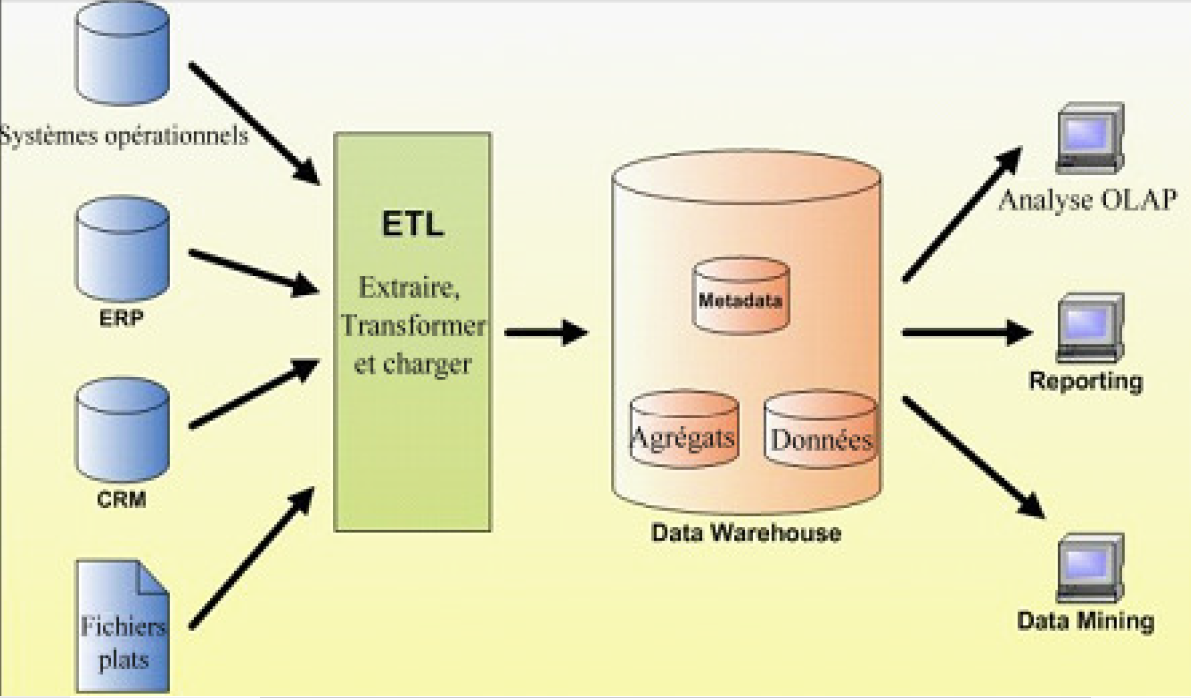
\includegraphics[scale=0.85]{images/DataWH.png}
		\caption{Architecture generale d'un data warehouse}
		\label{architecture-data-warehouse}
	\end{center}
\end{figure}

La figure ci-dessus Illustre la forme générale d’un data Warehouse que nous allons détailler dans les paragraphes suivants.

\textbf{Les Sources de données :} Dans la figure, les représentations de systèmes opérationnel, ERP, CRM et Fichiers plat font office de source de données et c’est d’elles qu’on puisse les données pour alimenter la machine décisionnelle.

\textbf{ETL (Extract, Transform, Load)}: C’est un ensemble de méthodes et d’outils qui servent a :\\
-	Extract : Extraire les données de sources hétérogènes\\
-	Transform : Transformation des données pour les mettre dans un format acceptable\\
-	Load : Charger les données dans le data warehouse\\

\textbf{Data Warehouse} : L’unité de stockage des données. Il est constitué de plusieurs éléments dont :\\ 
-	\textbf{Meta données} : ce sont les informations relatives à la structure des données, les méthodes d’agrégation et le lien entre les données opérationnelles et celles du Data Warehouse. Les métadonnées doivent renseigner sur :
 \begin{description}
 \item Le modèle de données,
 \item La structure des données telle qu’elle est vue par les développeurs,
 \item La structure des données telle qu’elle est vue par les utilisateurs,
 \item Les sources des données,
 \item Les transformations nécessaires,
 \item Suivi des alimentations,
 \end{description}
-	\textbf{Les Agrégats} (Données agrégées) : données agrégées à partir des données détaillées.\\

Les derniers éléments de la figure font partie de la phase d’exploitation du data warehouse et seront détaillés plus bas dans le document.


\section{Modélisation des données de l’entrepôt}

 \subsection{La modélisation dimensionnelle et ses concepts}
 	Les Data Warehouse sont destinés à la mise en place de systèmes décisionnels. Ces systèmes, devant répondre à des objectifs différents des systèmes transactionnels, ont fait ressortir très vite la nécessité de recourir à un modèle de données simplifié et aisément compréhensible. La modélisation dimensionnelle permet cela. Elle consiste à considérer un sujet d’analyse comme un cube à plusieurs dimensions, offrant des vues en tranches ou des analyses selon différents axes.
 	
 \begin{figure}[h]
	\begin{center}
		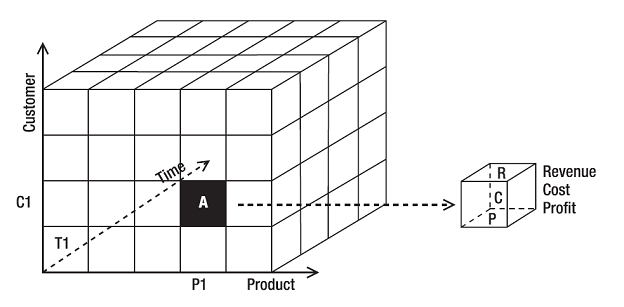
\includegraphics[scale=0.85]{images/cube.png}
		\caption{A cube with three dimensions.[ Rainardi 2008].}
		\label{Cube-dimensionnel}
	\end{center}
\end{figure}
 
 
 \subsubsection{Le concept des Faits}
 	 Une table de faits est la table centrale d’un modèle dimensionnel, où les mesures de performances sont stockées. Une ligne d'une table de faits correspond à une mesure. Ces mesures sont généralement des valeurs numériques, additives ; cependant des mesures textuelles peuvent exister mais sont rares. Le concepteur doit faire son possible pour faire des mesures textuelles des dimensions, car elles peuvent êtres corrélées efficacement avec les autres attributs textuels de dimensions.
 
 \subsubsection{Le concept des Dimensions}
 
  Les tables de dimension sont les tables qui raccompagnent une table de faits, elles contiennent les descriptions textuelles de l'activité. Une table de dimension est constituée de nombreuses colonnes qui décrivent une ligne. C'est grâce à cette table que l'entrepôt de données est compréhensible et utilisable; elles permettent des analyses en tranches et en dés. Une dimension est généralement constituée : d'une clé artificielle, une clé naturelle et des attributs.
  
 \subsection{Différents modèles de la modélisation dimensionnelle}
  
  \textbf{Modèle en étoile} : comme indiqué précédemment, ce modèle se présente comme une étoile dont le centre n’est autre que la table des faits et les branches sont les tables de dimension. La force de ce type de modélisation est sa lisibilité et sa performance. 
  
  \begin{figure}[h]
	\begin{center}
		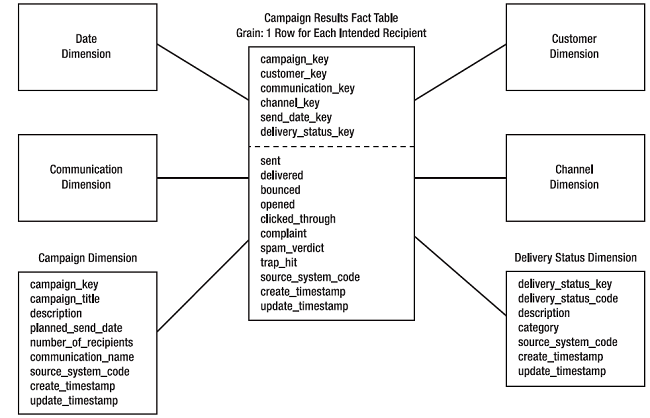
\includegraphics[scale=0.85]{images/etoile.png}
		\caption{Exemple d'un modèle en étoile « Dimensional star schema for campaign results data mart »[ Rainardi 2008]}
		\label{model-en-etoile}
	\end{center}
\end{figure}
\textbf{Modèle en flocon} : identique au modèle en étoile, sauf que ses branches sont éclatées en hiérarchies. Cette modélisation est généralement justifiée par l'économie d'espace de stockage, cependant elle peut s’avérer moins compréhensible pour l'utilisateur final, et très couteux en termes de performances.

\textbf{Modèle en constellation} : Ce n'est rien d'autre que plusieurs modèles en étoile liés entre eux par des dimensions communes.

  
  \subsection{La navigation dans les données}
  
  \paragraph{}
  Une fois que le serveur OLAP a construit le cube multidimensionnel « ou simulé ce cube selon l’architecture du serveur », plusieurs opérations sont possibles sur ce dernier offrant ainsi la possibilité de naviguer dans les données qui le constituent. Ces opérations de navigation « Data Surfing » doivent être, d’une part, assez complexes pour adresser l’ensemble des données et, d’autre part, assez simples afin de permettre à l’utilisateur de circuler de manière libre et intuitive dans le modèle dimensionnel.\\
  
Afin de répondre à ces attentes, un ensemble de mécanismes est exploité, permettant une navigation par rapport à la dimension et par rapport à la granularité d’une dimension.

  \subsubsection{Slice \& Dice}
  Le « Slicing » et le « Dicing » sont des techniques qui offrent la possibilité de faire des tranches « trancher » dans les données par rapport à des filtres de dimension bien précis, se classant de fait comme des opérations liées à la structure « se font sur les dimensions ». La différence entre eux se manifestent dans le fait que :\\
  
  \textit{Slicing is the process of retrieving a block of data from a cube by filtering on one dimension [Rainardi 2008].} 
   
   \begin{figure}[h]
	\begin{center}
		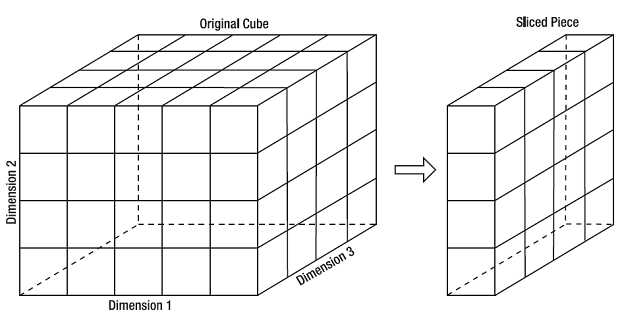
\includegraphics[scale=0.85]{images/slicing.png}
		\caption{Slicing}
		\label{slicing-image}
	\end{center}
   \end{figure}

\textit{Dicing is the process of retrieving a block of data from a cube by filtering on all dimensions [Rainardi 2008].}
  
    \begin{figure}[h]
	\begin{center}
		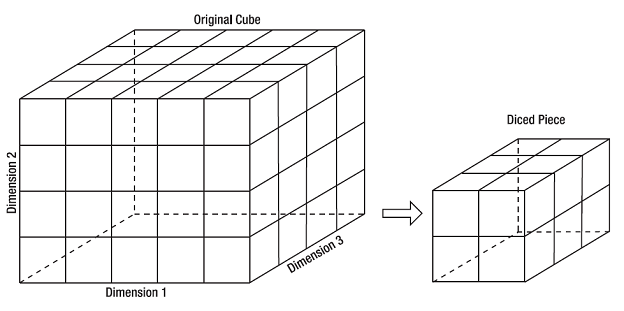
\includegraphics[scale=0.85]{images/dicing.png}
		\caption{Dicing}
		\label{slicing-image}
	\end{center}
   \end{figure}
   
   
   
\section{Démarche de Construction d’un Data Warehouse}   
   Plusieurs chercheurs ou équipes de recherche ont essayé de proposer des démarches pour la réalisation d’un projet Data Warehouse, ces démarches se croisent essentiellement dans les étapes suivantes :
\begin{list}{•}{ }
   \item Modélisation et conception du Data Warehouse,
   \item Alimentation du Data Warehouse,
   \item Mise en œuvre du Data Warehouse,
   \item Administration et maintenance du Data Warehouse,\\
\end{list}

\subsection{Modélisation et conception du Data Warehouse}

Les deux approches les plus connues dans la conception des Data Warehouse sont :
\begin{list}{•}{ }
   \item L’approche basée sur les besoins d’analyse,
    \item L’approche basée sur les sources de données,\\
\end{list}
Aucune des deux approches citées n’est ni parfaite, ni applicable à tous les cas. Toutes deux doivent être étudiées pour choisir celle qui s’adapte le mieux à notre cas. Quel que soit l’approche adoptée pour la conception d’un Data Warehouse, la définition de celui-là reste la même. En étant un support d’aide à la décision, le Data Warehouse se base sur une architecture dimensionnelle.


 \subsubsection{Approche « Besoins d’analyse »}
 
  Le contenu du Data Warehouse sera déterminé selon les besoins de l’utilisateur final. Cette approche est aussi appelée « approche descendante » (Top-Down Approach) et est illustrée par R. Kimball grâce à son cycle de vie dimensionnel comme suit :
  
  \begin{figure}[h]
	\begin{center}
		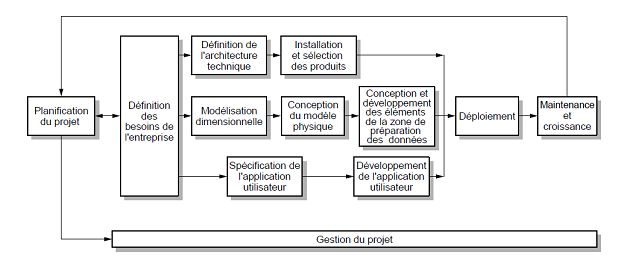
\includegraphics[scale=0.85]{images/besion_analyse.png}
		\caption{illustration de l’approche « Besoins d’analyse » grâce au cycle de vie dimensionnel de Kimball [Kimball, 2004].}
		\label{synthese-cout-salarie}
	\end{center}
\end{figure}

\begin{flushleft}
	\begin{longtable}{|p{0.5\textwidth}|p{0.5\textwidth}|}
		\caption{Avantages et inconvénients de l'approche « Besoins d’analyse »} 
		\label{Transactionel vs descisionel}
		\\
		
		
		\hline 
		\textbf{Avantages} &
		\textbf{Inconvénients}
		\\
		
		\hline
		\endhead
		\hline
		\endfoot
		\hline
		 
		\begin{description}
		 \item Aucun risque de concevoir une solution obsolète avant d’être opérationnelle
		 \end{description}
		  &
		 
	   \begin{description}
		\item  Pas de prise en compte de l’évolution des besoins de l’utilisateur.
		\item Nécessite une modification de la structure du Data Warehouse en cas de nouveau besoin
		\item Négligence du système opérationnel
		\item Difficulté de déterminer les besoins des utilisateurs
		\end{description}
		\\ 	
		\hline 
	\end{longtable} 
\end{flushleft}


\subsubsection{Approche « Source de données »}
Le contenu du Data Warehouse est déterminé selon les sources de données. Cette approche est appelée: Approche ascendante (Bottom-up Approach).

  \begin{flushleft}
	\begin{longtable}{|p{0.5\textwidth}|p{0.5\textwidth}|}
		\caption{Avantages et inconvénients de l'approche « Besoins d’analyse »} 
		\label{Transactionel vs descisionel}
		\\
		
		
		\hline 
		\textbf{Avantages} &
		\textbf{Inconvénients}
		\\
		
		\hline
		\endhead
		\hline
		\endfoot
		\hline
		 
		\begin{description}
		 \item Meilleure prise en charge de l’évolution des besoins
		 \end{description}
		  &
		 
	   \begin{description}
		\item  Risque de concevoir une solution obsolète avant qu’elle soit opérationnelle
		\item Evolution du schéma des données source
		\item Complexité de source de données
		\end{description}
		\\ 	
		\hline 
	\end{longtable} 
\end{flushleft}


\paragraph{•}
Inmon considère que l’utilisateur ne peut jamais déterminer ses besoins dès le départ, « Donnez-moi ce que je vous demande, et je vous direz ce dont j’ai vraiment besoin », il considère que les besoins sont en constante évolution.

\subsubsection{Approche mixte}
\paragraph{}
Une combinaison des deux approches appelée hybride ou mixte peut s’avérer efficace. Elle prend en considération les sources de données et les besoins des utilisateurs.\\

Cette approche consiste à construire des schémas dimensionnels à partir des structures des données du système opérationnel, et les valider par rapport aux besoins analytiques. Cette approche cumule les avantages et quelques inconvénients des deux approches déjà citées, telles que la complexité des sources de données et la difficulté quant à la détermination des besoins analytiques.


\subsection{Les phases de l'alimentation « E.T.L »}

Les phases du processus E.T.L. représentent la mécanique d’alimentation du Data
Warehouse. Ainsi elles se déroulent comme suit :\\
\textbf{a) L’extraction des données}\\

\textit{« L’extraction est la première étape du processus d’apport de données à l’entrepôt de données. Extraire, cela veut dire lire et interpréter les données sources et les copier dans la zone de préparation en vue de manipulations ultérieures. »} [Kimball, 2005]. Elle consiste en :\\

 •	Cibler les données,\\
 •	Appliquer les filtres nécessaires,\\
 •	Définir la fréquence de chargement\\

Lors du chargement des données, il faut extraire les nouvelles données ainsi que les changements intervenus sur ces données. Pour cela, il existe trois stratégies de capture de changement :\\
• Colonnes d’audit : la colonne d’audit, est une colonne qui enregistre la date d’insertion ou du dernier changement d’un enregistrement. Cette colonne est mise à jour soit par des triggers ou par les applications opérationnelles, d’où la nécessité de vérifier leur fiabilité.\\
\quad •	Capture des logs : certains outils ETL utilisent les fichiers logs des systèmes sources afin de détecter les changements (généralement logs du SGBD). En plus de l’absence de cette fonctionnalité sur certains outils ETL du marché, l’effacement des fichiers logs engendre la perte de toute information relative aux transactions.\\
\qquad • Comparaison avec le dernier chargement : le processus d’extraction sauvegarde des copies des chargements antérieurs, de manière à procéder à une comparaison lors de chaque nouvelle extraction. Il est impossible de rater un nouvel enregistrement avec cette méthode.


\begin{figure}[h]
	\begin{center}
		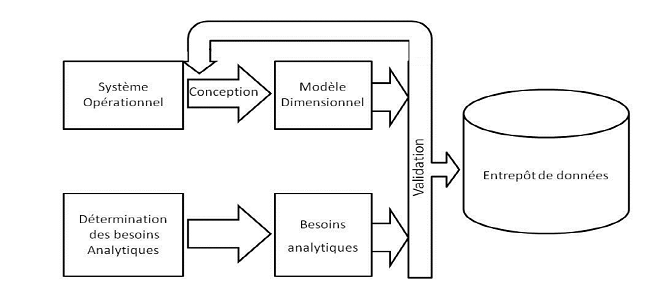
\includegraphics[scale=0.85]{images/mixte.png}
		\caption{Illustration de l’approche mixte.}
		\label{synthese-cout-salarie}
	\end{center}
\end{figure}

\textbf{b) La transformation des données}

La transformation est la seconde phase du processus. Cette étape, qui du reste est très importante, assure en réalité plusieurs tâches qui garantissent la fiabilité des données et leurs qualités. Ces tâches sont :\\
•	Consolidation des données.\\
•	Correction des données et élimination de toute ambiguïté.\\
•	Élimination des données redondantes.\\
•	Compléter et renseigner les valeurs manquantes. Cette opération se solde par la production d’informations dignes d’intérêt pour l’entreprise et de et sont donc prêtes à être entreposées.\\

\textbf{c) Le chargement des données}

C’est la dernière phase de l’alimentation d’un entrepôt de données, le chargement est une étape indispensable. Elle reste toutefois très délicate et exige une certaine connaissance des structures du système de gestion de la base de données (tables et index) afin d’optimiser au mieux le processus.

\subsubsection{Politiques de l’alimentation}
\paragraph{}
Le processus de l’alimentation peut se faire de différentes manières. Le choix de la politique de chargement dépend des sources : disponibilité et accessibilité. Ces politiques
sont8 :\\
\textbf{• Push} : dans cette méthode, la logique de chargement est dans le système de production. Il " pousse " les données vers la zone de préparation quand il en a l'occasion. L'inconvénient est que si le système est occupé, il ne poussera jamais les données.\\
\textbf{• Pull} : contrairement de la méthode précédente, le Pull " tire " les données de la source vers la zone de préparation. L'inconvénient de cette méthode est qu'elle peut surcharger le système s'il est en cours d'utilisation.\\
\textbf{• Push-pull} : c'est la combinaison des deux méthodes. La source prépare les données à envoyer et indique à la zone de préparation qu'elle est prête. La zone de préparation va alors récupérer les données.
Les Processus ETL doit respecter les critères suivants\\
\textbf{Sûr }: assure l’acheminement des données et leur livraison.
Rapide : la quantité de données manipulées peut causer des lenteurs. Le processus d’alimentation doit palier à ce problème et assurer le chargement du Data Warehouse dans des délais acceptables.\\
\textbf{Correctif }: le processus d’alimentation doit apporter les correctifs nécessaires pour améliorer la qualité des données.\\
\textbf{Transparent} : le processus de l’ETL doit être transparent afin d’améliorer la qualité des données.


\subsection{Mise en œuvre du Data Warehouse}
  C’est la dernière étape d’un projet Data Warehouse, soit son exploitation. L’exploitation du Data Warehouse se fait par le biais d’un ensemble d’outils analytiques développés autour du Data Warehouse. Donc cette étape nécessite l’achèvement du développement, ou de la mise en place, de ces outils qui peuvent accomplir les fonctions suivantes:\\
  
 \textbf{a. Requêtage ad-hoc}\\ 
  Le requêtage ad-hoc reste très fréquent dans ce type de projet. En effet, les utilisateurs de l’entrepôt de données, et spécialement les analystes, seront amenés à interagir avec le DW via des requêtes ad-hoc dans le but de faire les analyses requises par leurs métiers et, d’élaborer aussi, des rapports et des tableaux de bords spécifiques. L’accès à ce genre de service peut se faire via différentes méthodes et outils. Cependant, les spécialistes en la matière préconisent de laisser la possibilité à l’utilisateur de choisir les outils qui lui paraissent les plus adéquats.
  
 \textbf{ b. Reporting :}\\
Destiné essentiellement à la production de rapports et de tableaux de bord, \textit{« il est la présentation périodique de rapports sur les activités et résultats d'une organisation, d'une unité de travail ou du responsable d'une fonction, destinée à en informer ceux chargés de les superviser en interne ou en externe, ou tout simplement concernés par ces activités ou résultants »[ http://fr.wikipedia.org/wiki/Reporting].}\\

Ces outils de Reporting ne sont pas, à proprement parler, des instruments d'aide à la décision, mais, lorsqu’ils sont utilisés de manière appropriée, ils peuvent fournir une précieuse vue d’ensemble.\\

Les rapports sont alors crées par le biais d’outils de Reporting qui permettent de leur donner un format prédéterminé. Les requêtes sont constituées lors de l’élaboration des rapports qui seront ensuite diffusés périodiquement en automatique ou ponctuellement à la demande.\\


\textbf{d. Tableaux de bord :}\\
Les tableaux de bord sont un outil de pilotage qui donne une vision sur l’évolution d’un processus, afin de permettre aux responsables de mettre en place des actions correctives.\\
\textit{« Le tableau de bord est un ensemble d’indicateurs peu nombreux conçus pour permettre aux gestionnaires de prendre connaissance de l’état et de l’évolution des systèmes qu’ils pilotent et d’identifier les tendances qui les influenceront sur un horizon cohérent avec la nature de leurs fonctions » [Bouquin, 2003]}.\\
Cette forme de restitution a la particularité de se limiter à l’essentiel, c'est-à-dire la mise en évidence de l’état d’un indicateur par rapport à un objectif, tout en adoptant une représentation graphique de l’information.\\

\textbf{e. Data Mining :}\\
Au sens littéral du terme, le Data Mining signifie le forage de données. Le but de ce forage est d’extraire de la matière brute qui, dans notre cas, représente de nouvelles connaissances. L’idée de départ veut qu’il existe dans toute entreprise des connaissances utiles, cachées sous des gisements de données. Le Data Mining permet donc, grâce à un certain nombre de techniques, de découvrir ces connaissances en faisant apparaître des corrélations entre ces données.\\
Le Data Warehouse constituera alors la première source de données sur laquelle s’exécutera le processus de découverte de connaissances. Dans la majeure partie du temps, l’entrepôt de données représente un pré requis indispensable à toute fouille de données.\\
Le recours à ce genre de méthode est de plus en plus utilisé dans les entreprises modernes. Les applications et outils implémentant ces solutions sont rarement développés en interne. En effet, les entreprises préfèrent se reposer sur des valeurs sûres du marché afin d’exploiter au plus vite les données en leur possession.

 \subsection{Maintenance et expansion}
 La mise en service du Data Warehouse ne signifie pas la fin du projet, car un projet
Data Warehouse nécessite un suivi constant compte tenu des besoins d’optimisation de performance et ou d’expansion. Il est donc nécessaire d’investir dans les domaines suivants:\\
\textbf{Support} : assurer un support aux utilisateurs pour leur faire apprécier l’utilisation de l’entrepôt de données. En outre, la relation directe avec les utilisateurs permet de détecter les  correctifs nécessaires à apporter.\\
\textbf{Formation} : il est indispensable d’offrir un programme de formation permanant aux utilisateurs de l’entrepôt de données.\\
Support technique : un entrepôt de données est considéré comme un environnement de production. Naturellement le support technique doit surveiller avec la plus grande vigilance les performances et les tendances en ce qui concerne la charge du système.\\
\textbf{Management de l’évolution}: il faut toujours s’assurer que l’implémentation répond aux besoins de l’entreprise. Les revues systématiques à certain point de contrôle sont un outil clé pour détecter et définir les possibilités d’amélioration. En plus du suivi et de la maintenance du Data Warehouse, des demandes d’expansion sont envisageables pour de nouveaux besoins, de nouvelles données ou pour des améliorations.
Ces travaux d’expansion sont à prévoir de façon à faciliter l’évolution du schéma du
Data Warehouse.


%\begin{figure}[h]
%	\begin{center}
%		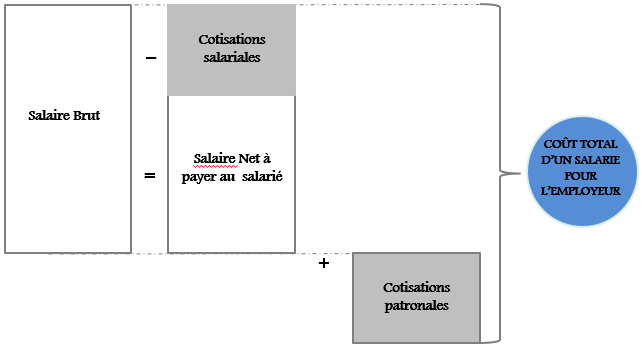
\includegraphics[scale=0.85]{images/remuneration.png}
%		\caption{Schéma de synthèse sur le coût d'un salarié}
%		\label{synthese-cout-salarie}
%	\end{center}
%\end{figure}


             % chapitre 1
\chapter{Titre du chapitre}     % numéroté

Texte du chapitre.
             % chapitre 2, etc.
\chapter*{Conclusion}
\addcontentsline{toc}{chapter}{Conclusion}

            % conclusion

\appendix                       % annexes le cas échéant

\chapter{Titre de l'annexe}     % numérotée

Texte de l'annexe.
                % annexe A

\bibliography{}                 % production de la bibliographie

\end{document}
%</gabarit>
%
% ^^A Gabarits des parties du document
%<*resume>
\chapter*{Résumé}                      % ne pas numéroter
\phantomsection\addcontentsline{toc}{chapter}{Résumé} % inclure dans TdM

\begin{otherlanguage*}{french}
  Texte du résumé en français.
\end{otherlanguage*}
%</resume>
%
%<*abstract>
\chapter*{Abstract}                      % ne pas numéroter
\phantomsection\addcontentsline{toc}{chapter}{Abstract} % inclure dans TdM

\begin{otherlanguage*}{english}
  Text of English abstract.
\end{otherlanguage*}
%</abstract>
%
%<*remerciements>
\chapter*{Remerciements}         % ne pas numéroter
\phantomsection\addcontentsline{toc}{chapter}{Remerciements} % inclure dans TdM

Texte des remerciements en prose.
%</remerciements>
%
%<*avantpropos>
\chapter*{Avant-propos}         % ne pas numéroter
\phantomsection\addcontentsline{toc}{chapter}{Avant-propos} % inclure dans TdM

L'avant-propos est surtout nécessaire pour une thèse par article.
%</avantpropos>
%
%<*introduction>
\chapter*{Introduction}         % ne pas numéroter
\phantomsection\addcontentsline{toc}{chapter}{Introduction} % inclure dans TdM

Une thèse ou un mémoire devrait normalement débuter par une
introduction. Celle-ci est traitée comme un chapitre normal, sauf
qu'elle n'est pas numérotée.
%</introduction>
%
%<*chapitre>
\chapter{Titre du chapitre}     % numéroté

Texte du chapitre.
%</chapitre>
%
%<*conclusion>
\chapter*{Conclusion}         % ne pas numéroter
\phantomsection\addcontentsline{toc}{chapter}{Conclusion} % dans TdM

Une thèse ou un mémoire devrait normalement se terminer par une
conclusion, placée avant les annexes, le cas échéant. Celle-ci est
traitée comme un chapitre normal, sauf qu'elle n'est pas numérotée.
%</conclusion>
%
%<*annexe>
\chapter{Titre de l'annexe}     % numérotée

Texte de l'annexe.
%</annexe>
% Local Variables:
% mode: doctex
% coding: utf-8
% TeX-master: t
% TeX-engine: xetex
% End:
% \fi
